% Options for packages loaded elsewhere
\PassOptionsToPackage{unicode}{hyperref}
\PassOptionsToPackage{hyphens}{url}
%
\documentclass[
]{article}
\usepackage{amsmath,amssymb}
\usepackage{iftex}
\ifPDFTeX
  \usepackage[T1]{fontenc}
  \usepackage[utf8]{inputenc}
  \usepackage{textcomp} % provide euro and other symbols
\else % if luatex or xetex
  \usepackage{unicode-math} % this also loads fontspec
  \defaultfontfeatures{Scale=MatchLowercase}
  \defaultfontfeatures[\rmfamily]{Ligatures=TeX,Scale=1}
\fi
\usepackage{lmodern}
\ifPDFTeX\else
  % xetex/luatex font selection
\fi
% Use upquote if available, for straight quotes in verbatim environments
\IfFileExists{upquote.sty}{\usepackage{upquote}}{}
\IfFileExists{microtype.sty}{% use microtype if available
  \usepackage[]{microtype}
  \UseMicrotypeSet[protrusion]{basicmath} % disable protrusion for tt fonts
}{}
\makeatletter
\@ifundefined{KOMAClassName}{% if non-KOMA class
  \IfFileExists{parskip.sty}{%
    \usepackage{parskip}
  }{% else
    \setlength{\parindent}{0pt}
    \setlength{\parskip}{6pt plus 2pt minus 1pt}}
}{% if KOMA class
  \KOMAoptions{parskip=half}}
\makeatother
\usepackage{xcolor}
\usepackage[margin=1in]{geometry}
\usepackage{color}
\usepackage{fancyvrb}
\newcommand{\VerbBar}{|}
\newcommand{\VERB}{\Verb[commandchars=\\\{\}]}
\DefineVerbatimEnvironment{Highlighting}{Verbatim}{commandchars=\\\{\}}
% Add ',fontsize=\small' for more characters per line
\usepackage{framed}
\definecolor{shadecolor}{RGB}{248,248,248}
\newenvironment{Shaded}{\begin{snugshade}}{\end{snugshade}}
\newcommand{\AlertTok}[1]{\textcolor[rgb]{0.94,0.16,0.16}{#1}}
\newcommand{\AnnotationTok}[1]{\textcolor[rgb]{0.56,0.35,0.01}{\textbf{\textit{#1}}}}
\newcommand{\AttributeTok}[1]{\textcolor[rgb]{0.13,0.29,0.53}{#1}}
\newcommand{\BaseNTok}[1]{\textcolor[rgb]{0.00,0.00,0.81}{#1}}
\newcommand{\BuiltInTok}[1]{#1}
\newcommand{\CharTok}[1]{\textcolor[rgb]{0.31,0.60,0.02}{#1}}
\newcommand{\CommentTok}[1]{\textcolor[rgb]{0.56,0.35,0.01}{\textit{#1}}}
\newcommand{\CommentVarTok}[1]{\textcolor[rgb]{0.56,0.35,0.01}{\textbf{\textit{#1}}}}
\newcommand{\ConstantTok}[1]{\textcolor[rgb]{0.56,0.35,0.01}{#1}}
\newcommand{\ControlFlowTok}[1]{\textcolor[rgb]{0.13,0.29,0.53}{\textbf{#1}}}
\newcommand{\DataTypeTok}[1]{\textcolor[rgb]{0.13,0.29,0.53}{#1}}
\newcommand{\DecValTok}[1]{\textcolor[rgb]{0.00,0.00,0.81}{#1}}
\newcommand{\DocumentationTok}[1]{\textcolor[rgb]{0.56,0.35,0.01}{\textbf{\textit{#1}}}}
\newcommand{\ErrorTok}[1]{\textcolor[rgb]{0.64,0.00,0.00}{\textbf{#1}}}
\newcommand{\ExtensionTok}[1]{#1}
\newcommand{\FloatTok}[1]{\textcolor[rgb]{0.00,0.00,0.81}{#1}}
\newcommand{\FunctionTok}[1]{\textcolor[rgb]{0.13,0.29,0.53}{\textbf{#1}}}
\newcommand{\ImportTok}[1]{#1}
\newcommand{\InformationTok}[1]{\textcolor[rgb]{0.56,0.35,0.01}{\textbf{\textit{#1}}}}
\newcommand{\KeywordTok}[1]{\textcolor[rgb]{0.13,0.29,0.53}{\textbf{#1}}}
\newcommand{\NormalTok}[1]{#1}
\newcommand{\OperatorTok}[1]{\textcolor[rgb]{0.81,0.36,0.00}{\textbf{#1}}}
\newcommand{\OtherTok}[1]{\textcolor[rgb]{0.56,0.35,0.01}{#1}}
\newcommand{\PreprocessorTok}[1]{\textcolor[rgb]{0.56,0.35,0.01}{\textit{#1}}}
\newcommand{\RegionMarkerTok}[1]{#1}
\newcommand{\SpecialCharTok}[1]{\textcolor[rgb]{0.81,0.36,0.00}{\textbf{#1}}}
\newcommand{\SpecialStringTok}[1]{\textcolor[rgb]{0.31,0.60,0.02}{#1}}
\newcommand{\StringTok}[1]{\textcolor[rgb]{0.31,0.60,0.02}{#1}}
\newcommand{\VariableTok}[1]{\textcolor[rgb]{0.00,0.00,0.00}{#1}}
\newcommand{\VerbatimStringTok}[1]{\textcolor[rgb]{0.31,0.60,0.02}{#1}}
\newcommand{\WarningTok}[1]{\textcolor[rgb]{0.56,0.35,0.01}{\textbf{\textit{#1}}}}
\usepackage{graphicx}
\makeatletter
\def\maxwidth{\ifdim\Gin@nat@width>\linewidth\linewidth\else\Gin@nat@width\fi}
\def\maxheight{\ifdim\Gin@nat@height>\textheight\textheight\else\Gin@nat@height\fi}
\makeatother
% Scale images if necessary, so that they will not overflow the page
% margins by default, and it is still possible to overwrite the defaults
% using explicit options in \includegraphics[width, height, ...]{}
\setkeys{Gin}{width=\maxwidth,height=\maxheight,keepaspectratio}
% Set default figure placement to htbp
\makeatletter
\def\fps@figure{htbp}
\makeatother
\setlength{\emergencystretch}{3em} % prevent overfull lines
\providecommand{\tightlist}{%
  \setlength{\itemsep}{0pt}\setlength{\parskip}{0pt}}
\setcounter{secnumdepth}{5}
\ifLuaTeX
  \usepackage{selnolig}  % disable illegal ligatures
\fi
\usepackage{bookmark}
\IfFileExists{xurl.sty}{\usepackage{xurl}}{} % add URL line breaks if available
\urlstyle{same}
\hypersetup{
  pdftitle={Loan Approval},
  pdfauthor={Shaibu Abdullateef Topa (CST/20/COM/00591)},
  hidelinks,
  pdfcreator={LaTeX via pandoc}}

\title{Loan Approval}
\author{Shaibu Abdullateef Topa (CST/20/COM/00591)}
\date{2025-03-08}

\begin{document}
\maketitle

\#Load and inspect the dataset

\begin{Shaded}
\begin{Highlighting}[]
\CommentTok{\# Load data manipulation library}
\FunctionTok{library}\NormalTok{(dplyr)}

\CommentTok{\# Read the loan data set (same folder as this R script)}
\NormalTok{loan\_data }\OtherTok{\textless{}{-}} \FunctionTok{read.csv}\NormalTok{(}\StringTok{"loan\_approval.csv"}\NormalTok{)}
\end{Highlighting}
\end{Shaded}

\#Explore Dataset

\begin{Shaded}
\begin{Highlighting}[]
\CommentTok{\# Show first few rows}
\FunctionTok{head}\NormalTok{(loan\_data)}
\end{Highlighting}
\end{Shaded}

\begin{verbatim}
##   loan_id no_of_dependents     education self_employed income_annum loan_amount
## 1       1                2      Graduate            No      9600000    29900000
## 2       2                0  Not Graduate           Yes      4100000    12200000
## 3       3                3      Graduate            No      9100000    29700000
## 4       4                3      Graduate            No      8200000    30700000
## 5       5                5  Not Graduate           Yes      9800000    24200000
## 6       6                0      Graduate           Yes      4800000    13500000
##   loan_term cibil_score residential_assets_value commercial_assets_value
## 1        12         778                  2400000                17600000
## 2         8         417                  2700000                 2200000
## 3        20         506                  7100000                 4500000
## 4         8         467                 18200000                 3300000
## 5        20         382                 12400000                 8200000
## 6        10         319                  6800000                 8300000
##   luxury_assets_value bank_asset_value loan_status
## 1            22700000          8000000    Approved
## 2             8800000          3300000    Rejected
## 3            33300000         12800000    Rejected
## 4            23300000          7900000    Rejected
## 5            29400000          5000000    Rejected
## 6            13700000          5100000    Rejected
\end{verbatim}

\begin{Shaded}
\begin{Highlighting}[]
\CommentTok{\# Show last few rows}
\FunctionTok{tail}\NormalTok{(loan\_data)}
\end{Highlighting}
\end{Shaded}

\begin{verbatim}
##      loan_id no_of_dependents     education self_employed income_annum
## 4264    4264                3      Graduate            No      5000000
## 4265    4265                5      Graduate           Yes      1000000
## 4266    4266                0  Not Graduate           Yes      3300000
## 4267    4267                2  Not Graduate            No      6500000
## 4268    4268                1  Not Graduate            No      4100000
## 4269    4269                1      Graduate            No      9200000
##      loan_amount loan_term cibil_score residential_assets_value
## 4264    12700000        14         865                  4700000
## 4265     2300000        12         317                  2800000
## 4266    11300000        20         559                  4200000
## 4267    23900000        18         457                  1200000
## 4268    12800000         8         780                  8200000
## 4269    29700000        10         607                 17800000
##      commercial_assets_value luxury_assets_value bank_asset_value loan_status
## 4264                 8100000            19500000          6300000    Approved
## 4265                  500000             3300000           800000    Rejected
## 4266                 2900000            11000000          1900000    Approved
## 4267                12400000            18100000          7300000    Rejected
## 4268                  700000            14100000          5800000    Approved
## 4269                11800000            35700000         12000000    Approved
\end{verbatim}

\begin{Shaded}
\begin{Highlighting}[]
\CommentTok{\#Show the dataset dimension }
\FunctionTok{dim}\NormalTok{(loan\_data)}
\end{Highlighting}
\end{Shaded}

\begin{verbatim}
## [1] 4269   13
\end{verbatim}

\#Summary of dataset

\begin{Shaded}
\begin{Highlighting}[]
\CommentTok{\# Check dataset structure}
\FunctionTok{str}\NormalTok{(loan\_data)}
\end{Highlighting}
\end{Shaded}

\begin{verbatim}
## 'data.frame':    4269 obs. of  13 variables:
##  $ loan_id                 : int  1 2 3 4 5 6 7 8 9 10 ...
##  $ no_of_dependents        : int  2 0 3 3 5 0 5 2 0 5 ...
##  $ education               : chr  " Graduate" " Not Graduate" " Graduate" " Graduate" ...
##  $ self_employed           : chr  " No" " Yes" " No" " No" ...
##  $ income_annum            : int  9600000 4100000 9100000 8200000 9800000 4800000 8700000 5700000 800000 1100000 ...
##  $ loan_amount             : int  29900000 12200000 29700000 30700000 24200000 13500000 33000000 15000000 2200000 4300000 ...
##  $ loan_term               : int  12 8 20 8 20 10 4 20 20 10 ...
##  $ cibil_score             : int  778 417 506 467 382 319 678 382 782 388 ...
##  $ residential_assets_value: int  2400000 2700000 7100000 18200000 12400000 6800000 22500000 13200000 1300000 3200000 ...
##  $ commercial_assets_value : int  17600000 2200000 4500000 3300000 8200000 8300000 14800000 5700000 800000 1400000 ...
##  $ luxury_assets_value     : int  22700000 8800000 33300000 23300000 29400000 13700000 29200000 11800000 2800000 3300000 ...
##  $ bank_asset_value        : int  8000000 3300000 12800000 7900000 5000000 5100000 4300000 6000000 600000 1600000 ...
##  $ loan_status             : chr  " Approved" " Rejected" " Rejected" " Rejected" ...
\end{verbatim}

\begin{Shaded}
\begin{Highlighting}[]
\CommentTok{\# Summary statistics of the loan dataset}
\FunctionTok{summary}\NormalTok{(loan\_data)}
\end{Highlighting}
\end{Shaded}

\begin{verbatim}
##     loan_id     no_of_dependents  education         self_employed     
##  Min.   :   1   Min.   :0.000    Length:4269        Length:4269       
##  1st Qu.:1068   1st Qu.:1.000    Class :character   Class :character  
##  Median :2135   Median :3.000    Mode  :character   Mode  :character  
##  Mean   :2135   Mean   :2.499                                         
##  3rd Qu.:3202   3rd Qu.:4.000                                         
##  Max.   :4269   Max.   :5.000                                         
##   income_annum      loan_amount         loan_term     cibil_score   
##  Min.   : 200000   Min.   :  300000   Min.   : 2.0   Min.   :300.0  
##  1st Qu.:2700000   1st Qu.: 7700000   1st Qu.: 6.0   1st Qu.:453.0  
##  Median :5100000   Median :14500000   Median :10.0   Median :600.0  
##  Mean   :5059124   Mean   :15133450   Mean   :10.9   Mean   :599.9  
##  3rd Qu.:7500000   3rd Qu.:21500000   3rd Qu.:16.0   3rd Qu.:748.0  
##  Max.   :9900000   Max.   :39500000   Max.   :20.0   Max.   :900.0  
##  residential_assets_value commercial_assets_value luxury_assets_value
##  Min.   : -100000         Min.   :       0        Min.   :  300000   
##  1st Qu.: 2200000         1st Qu.: 1300000        1st Qu.: 7500000   
##  Median : 5600000         Median : 3700000        Median :14600000   
##  Mean   : 7472617         Mean   : 4973155        Mean   :15126306   
##  3rd Qu.:11300000         3rd Qu.: 7600000        3rd Qu.:21700000   
##  Max.   :29100000         Max.   :19400000        Max.   :39200000   
##  bank_asset_value   loan_status       
##  Min.   :       0   Length:4269       
##  1st Qu.: 2300000   Class :character  
##  Median : 4600000   Mode  :character  
##  Mean   : 4976692                     
##  3rd Qu.: 7100000                     
##  Max.   :14700000
\end{verbatim}

\begin{Shaded}
\begin{Highlighting}[]
\CommentTok{\# Check number of distinct values in the entire dataset}
\FunctionTok{sapply}\NormalTok{(loan\_data, }\ControlFlowTok{function}\NormalTok{(x) }\FunctionTok{length}\NormalTok{(}\FunctionTok{unique}\NormalTok{(x)))}
\end{Highlighting}
\end{Shaded}

\begin{verbatim}
##                  loan_id         no_of_dependents                education 
##                     4269                        6                        2 
##            self_employed             income_annum              loan_amount 
##                        2                       98                      378 
##                loan_term              cibil_score residential_assets_value 
##                       10                      601                      278 
##  commercial_assets_value      luxury_assets_value         bank_asset_value 
##                      188                      379                      146 
##              loan_status 
##                        2
\end{verbatim}

\#From the above, categorical feature :education, self\_emplyed and
loan\_status each has 2 unique values respectively
{[}Graduate,Not{]},{[}No,Yes{]},{[}Approved,Rejected{]}

\#Data Cleaning

\begin{Shaded}
\begin{Highlighting}[]
\CommentTok{\# Check for duplicates}
\FunctionTok{sum}\NormalTok{(}\FunctionTok{duplicated}\NormalTok{(loan\_data))}
\end{Highlighting}
\end{Shaded}

\begin{verbatim}
## [1] 0
\end{verbatim}

\#Handle Missing Values (if any)

\begin{Shaded}
\begin{Highlighting}[]
\CommentTok{\# Count missing values in each column}
\FunctionTok{colSums}\NormalTok{(}\FunctionTok{is.na}\NormalTok{(loan\_data))}
\end{Highlighting}
\end{Shaded}

\begin{verbatim}
##                  loan_id         no_of_dependents                education 
##                        0                        0                        0 
##            self_employed             income_annum              loan_amount 
##                        0                        0                        0 
##                loan_term              cibil_score residential_assets_value 
##                        0                        0                        0 
##  commercial_assets_value      luxury_assets_value         bank_asset_value 
##                        0                        0                        0 
##              loan_status 
##                        0
\end{verbatim}

\#Removed unnecessary spaces in column names and values

\begin{Shaded}
\begin{Highlighting}[]
\FunctionTok{names}\NormalTok{(loan\_data) }\OtherTok{\textless{}{-}} \FunctionTok{gsub}\NormalTok{(}\StringTok{" "}\NormalTok{, }\StringTok{""}\NormalTok{, }\FunctionTok{names}\NormalTok{(loan\_data))}
\end{Highlighting}
\end{Shaded}

\#Outlier mining

\begin{Shaded}
\begin{Highlighting}[]
\CommentTok{\#Detecting Outlier by Visualization}
\CommentTok{\# Load required libraries}
\FunctionTok{library}\NormalTok{(ggplot2)}
\FunctionTok{library}\NormalTok{(gridExtra)}

\CommentTok{\# Create empty list to store plots}
\NormalTok{plot\_list }\OtherTok{\textless{}{-}} \FunctionTok{list}\NormalTok{()}

\CommentTok{\# Create boxplot for each numeric column}
\NormalTok{num\_cols }\OtherTok{\textless{}{-}} \FunctionTok{sapply}\NormalTok{(loan\_data, is.numeric)}
\NormalTok{numeric\_data }\OtherTok{\textless{}{-}}\NormalTok{ loan\_data[, num\_cols]}

\CommentTok{\# Create individual boxplots}
\ControlFlowTok{for}\NormalTok{(col }\ControlFlowTok{in} \FunctionTok{names}\NormalTok{(numeric\_data)) \{}
\NormalTok{  p }\OtherTok{\textless{}{-}} \FunctionTok{ggplot}\NormalTok{(numeric\_data, }\FunctionTok{aes\_string}\NormalTok{(}\AttributeTok{y =}\NormalTok{ col)) }\SpecialCharTok{+} 
    \FunctionTok{geom\_boxplot}\NormalTok{() }\SpecialCharTok{+}
    \FunctionTok{labs}\NormalTok{(}\AttributeTok{title =}\NormalTok{ col) }\SpecialCharTok{+}
    \FunctionTok{theme\_minimal}\NormalTok{()}
  
\NormalTok{  plot\_list[[col]] }\OtherTok{\textless{}{-}}\NormalTok{ p}
\NormalTok{\}}

\CommentTok{\# Calculate grid dimensions (trying to approximate 4x4 layout)}
\NormalTok{n\_plots }\OtherTok{\textless{}{-}} \FunctionTok{length}\NormalTok{(plot\_list)}
\NormalTok{n\_rows }\OtherTok{\textless{}{-}} \FunctionTok{ceiling}\NormalTok{(}\FunctionTok{sqrt}\NormalTok{(n\_plots))}
\NormalTok{n\_cols }\OtherTok{\textless{}{-}} \FunctionTok{ceiling}\NormalTok{(n\_plots }\SpecialCharTok{/}\NormalTok{ n\_rows)}

\CommentTok{\# Arrange plots in a grid and display}
\FunctionTok{grid.arrange}\NormalTok{(}\AttributeTok{grobs =}\NormalTok{ plot\_list, }\AttributeTok{nrow =}\NormalTok{ n\_rows, }\AttributeTok{ncol =}\NormalTok{ n\_cols)}
\end{Highlighting}
\end{Shaded}

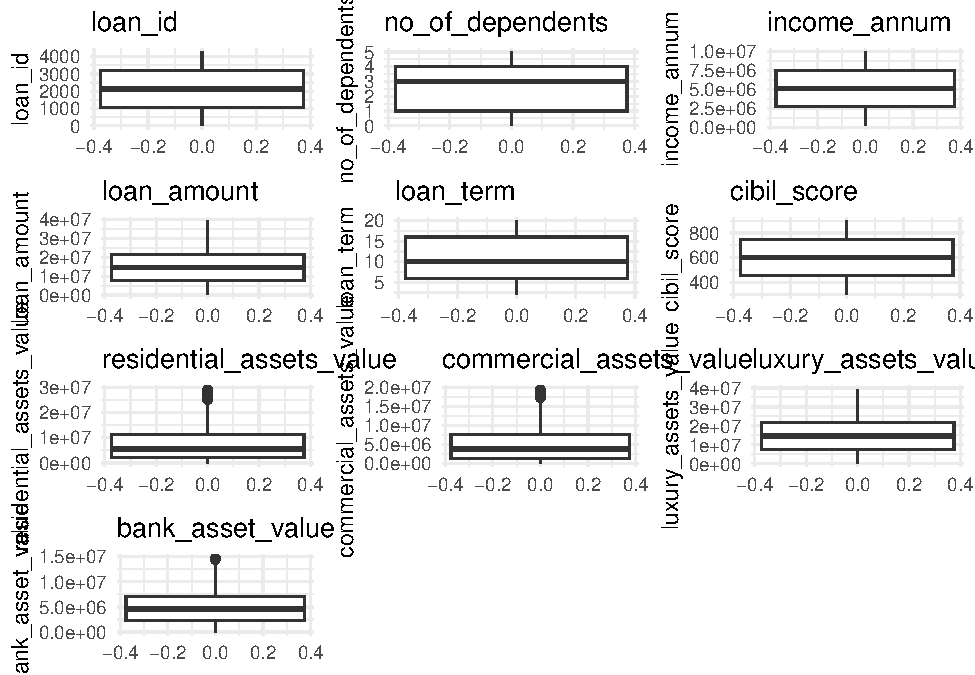
\includegraphics{Loan_approval_files/figure-latex/unnamed-chunk-10-1.pdf}

\#Outliers detected in features bank\_asset\_value: This indicates that
there are few applicants having more than 1,400,000 in their bank
accounts residental\_assets\_value and commercial\_assets\_value:
indicating there are few applicants having more value of residential and
commercial assets

\#Treating Outliers

\begin{Shaded}
\begin{Highlighting}[]
\CommentTok{\# Function to cap outliers}
\NormalTok{cap\_outliers }\OtherTok{\textless{}{-}} \ControlFlowTok{function}\NormalTok{(df, column, }\AttributeTok{method =} \StringTok{\textquotesingle{}IQR\textquotesingle{}}\NormalTok{) \{}
  \ControlFlowTok{if}\NormalTok{ (method }\SpecialCharTok{==} \StringTok{\textquotesingle{}IQR\textquotesingle{}}\NormalTok{) \{}
\NormalTok{    Q1 }\OtherTok{\textless{}{-}} \FunctionTok{quantile}\NormalTok{(df[[column]], }\FloatTok{0.25}\NormalTok{, }\AttributeTok{na.rm =} \ConstantTok{TRUE}\NormalTok{)}
\NormalTok{    Q3 }\OtherTok{\textless{}{-}} \FunctionTok{quantile}\NormalTok{(df[[column]], }\FloatTok{0.75}\NormalTok{, }\AttributeTok{na.rm =} \ConstantTok{TRUE}\NormalTok{)}
\NormalTok{    IQR\_val }\OtherTok{\textless{}{-}}\NormalTok{ Q3 }\SpecialCharTok{{-}}\NormalTok{ Q1}
\NormalTok{    lower\_bound }\OtherTok{\textless{}{-}}\NormalTok{ Q1 }\SpecialCharTok{{-}} \FloatTok{1.5} \SpecialCharTok{*}\NormalTok{ IQR\_val}
\NormalTok{    upper\_bound }\OtherTok{\textless{}{-}}\NormalTok{ Q3 }\SpecialCharTok{+} \FloatTok{1.5} \SpecialCharTok{*}\NormalTok{ IQR\_val}
\NormalTok{  \} }\ControlFlowTok{else} \ControlFlowTok{if}\NormalTok{ (method }\SpecialCharTok{==} \StringTok{\textquotesingle{}zscore\textquotesingle{}}\NormalTok{) \{}
\NormalTok{    mean\_val }\OtherTok{\textless{}{-}} \FunctionTok{mean}\NormalTok{(df[[column]], }\AttributeTok{na.rm =} \ConstantTok{TRUE}\NormalTok{)}
\NormalTok{    std\_val }\OtherTok{\textless{}{-}} \FunctionTok{sd}\NormalTok{(df[[column]], }\AttributeTok{na.rm =} \ConstantTok{TRUE}\NormalTok{)}
\NormalTok{    lower\_bound }\OtherTok{\textless{}{-}}\NormalTok{ mean\_val }\SpecialCharTok{{-}} \DecValTok{3} \SpecialCharTok{*}\NormalTok{ std\_val}
\NormalTok{    upper\_bound }\OtherTok{\textless{}{-}}\NormalTok{ mean\_val }\SpecialCharTok{+} \DecValTok{3} \SpecialCharTok{*}\NormalTok{ std\_val}
\NormalTok{  \}}
  
  \CommentTok{\# Cap the values using pmin/pmax (R\textquotesingle{}s equivalent to np.clip)}
\NormalTok{  df[[column]] }\OtherTok{\textless{}{-}} \FunctionTok{pmin}\NormalTok{(}\FunctionTok{pmax}\NormalTok{(df[[column]], lower\_bound), upper\_bound)}
  \FunctionTok{return}\NormalTok{(df)}
\NormalTok{\}}

\CommentTok{\# Apply to all numerical columns}
\NormalTok{num\_cols }\OtherTok{\textless{}{-}} \FunctionTok{sapply}\NormalTok{(loan\_data, is.numeric)}
\ControlFlowTok{for}\NormalTok{ (col }\ControlFlowTok{in} \FunctionTok{names}\NormalTok{(loan\_data[, num\_cols])) \{}
\NormalTok{  loan\_data }\OtherTok{\textless{}{-}} \FunctionTok{cap\_outliers}\NormalTok{(loan\_data, col, }\AttributeTok{method =} \StringTok{\textquotesingle{}IQR\textquotesingle{}}\NormalTok{)  }\CommentTok{\# or \textquotesingle{}zscore\textquotesingle{}}
\NormalTok{\}}

\FunctionTok{dim}\NormalTok{(loan\_data)}
\end{Highlighting}
\end{Shaded}

\begin{verbatim}
## [1] 4269   13
\end{verbatim}

\begin{Shaded}
\begin{Highlighting}[]
\CommentTok{\# Load necessary libraries}
\FunctionTok{library}\NormalTok{(ggplot2)}
\FunctionTok{library}\NormalTok{(gridExtra)}
\FunctionTok{library}\NormalTok{(ggpubr)}

\CommentTok{\# Boxplot}
\NormalTok{p1 }\OtherTok{\textless{}{-}} \FunctionTok{ggplot}\NormalTok{(loan\_data, }\FunctionTok{aes}\NormalTok{(}\AttributeTok{y =}\NormalTok{ commercial\_assets\_value)) }\SpecialCharTok{+}
  \FunctionTok{geom\_boxplot}\NormalTok{(}\AttributeTok{fill =} \StringTok{"skyblue"}\NormalTok{) }\SpecialCharTok{+}
  \FunctionTok{ggtitle}\NormalTok{(}\StringTok{"Boxplot"}\NormalTok{) }\SpecialCharTok{+}
  \FunctionTok{theme\_minimal}\NormalTok{()}

\CommentTok{\# Histogram with density curve {-} using after\_stat() instead of ..density..}
\NormalTok{p2 }\OtherTok{\textless{}{-}} \FunctionTok{ggplot}\NormalTok{(loan\_data, }\FunctionTok{aes}\NormalTok{(}\AttributeTok{x =}\NormalTok{ commercial\_assets\_value)) }\SpecialCharTok{+}
  \FunctionTok{geom\_histogram}\NormalTok{(}\FunctionTok{aes}\NormalTok{(}\AttributeTok{y =} \FunctionTok{after\_stat}\NormalTok{(density)), }\AttributeTok{bins =} \DecValTok{30}\NormalTok{, }\AttributeTok{fill =} \StringTok{"skyblue"}\NormalTok{, }\AttributeTok{color =} \StringTok{"black"}\NormalTok{, }\AttributeTok{alpha =} \FloatTok{0.7}\NormalTok{) }\SpecialCharTok{+}
  \FunctionTok{geom\_density}\NormalTok{(}\AttributeTok{color =} \StringTok{"red"}\NormalTok{, }\AttributeTok{linewidth =} \DecValTok{1}\NormalTok{) }\SpecialCharTok{+}
  \FunctionTok{ggtitle}\NormalTok{(}\StringTok{"Histogram with Density"}\NormalTok{) }\SpecialCharTok{+}
  \FunctionTok{theme\_minimal}\NormalTok{()}

\CommentTok{\# Q{-}Q plot}
\NormalTok{p3 }\OtherTok{\textless{}{-}} \FunctionTok{ggplot}\NormalTok{(loan\_data, }\FunctionTok{aes}\NormalTok{(}\AttributeTok{sample =}\NormalTok{ commercial\_assets\_value)) }\SpecialCharTok{+}
  \FunctionTok{stat\_qq}\NormalTok{() }\SpecialCharTok{+}
  \FunctionTok{stat\_qq\_line}\NormalTok{() }\SpecialCharTok{+}
  \FunctionTok{ggtitle}\NormalTok{(}\StringTok{"Q{-}Q Plot"}\NormalTok{) }\SpecialCharTok{+}
  \FunctionTok{theme\_minimal}\NormalTok{()}

\CommentTok{\# Combine all plots}
\FunctionTok{grid.arrange}\NormalTok{(p1, p2, p3, }\AttributeTok{ncol =} \DecValTok{3}\NormalTok{)}
\end{Highlighting}
\end{Shaded}

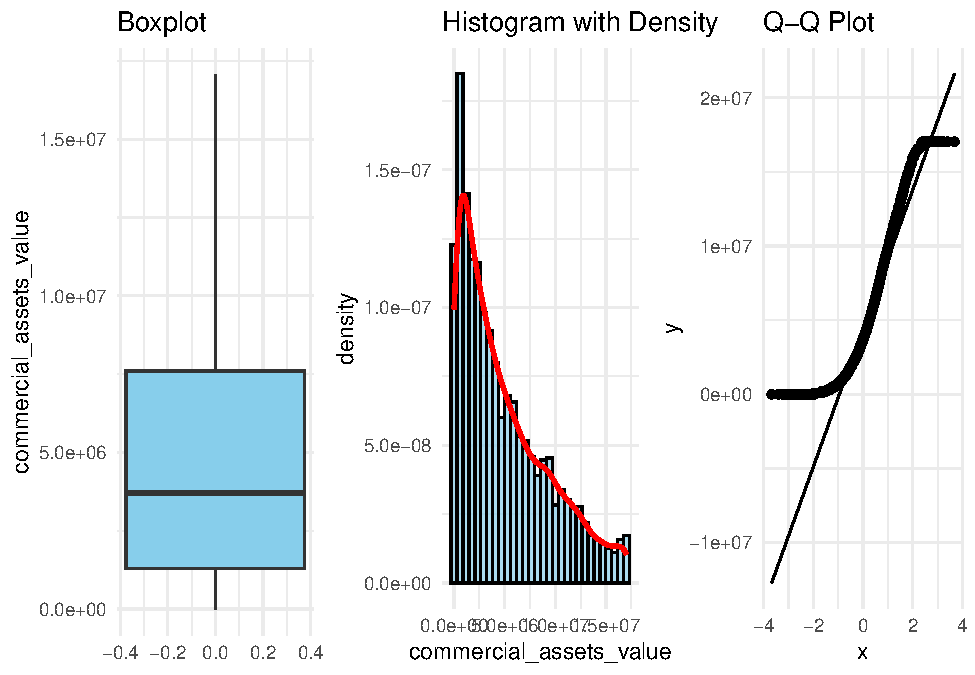
\includegraphics{Loan_approval_files/figure-latex/unnamed-chunk-12-1.pdf}

\section{Exploratory Data Analysis
(EDA)}\label{exploratory-data-analysis-eda}

\begin{Shaded}
\begin{Highlighting}[]
\FunctionTok{library}\NormalTok{(ggplot2)}
\FunctionTok{library}\NormalTok{(reshape2)}

\CommentTok{\# Correlation Between Features}


\CommentTok{\# First, clean the spaces in character columns}
\NormalTok{loan\_data\_clean }\OtherTok{\textless{}{-}}\NormalTok{ loan\_data}
\NormalTok{char\_cols }\OtherTok{\textless{}{-}} \FunctionTok{sapply}\NormalTok{(loan\_data, is.character)}

\ControlFlowTok{for}\NormalTok{ (col }\ControlFlowTok{in} \FunctionTok{names}\NormalTok{(loan\_data)[char\_cols]) \{}
\NormalTok{  loan\_data\_clean[[col]] }\OtherTok{\textless{}{-}} \FunctionTok{trimws}\NormalTok{(loan\_data\_clean[[col]])}
\NormalTok{\}}

\CommentTok{\# Make a copy for correlation}
\NormalTok{loan\_data\_corr }\OtherTok{\textless{}{-}}\NormalTok{ loan\_data\_clean}

\CommentTok{\# Encode binary categorical variables}
\NormalTok{binary\_cats }\OtherTok{\textless{}{-}} \FunctionTok{c}\NormalTok{(}\StringTok{\textquotesingle{}education\textquotesingle{}}\NormalTok{, }\StringTok{\textquotesingle{}self\_employed\textquotesingle{}}\NormalTok{, }\StringTok{\textquotesingle{}loan\_status\textquotesingle{}}\NormalTok{)}
\NormalTok{encoding\_map }\OtherTok{\textless{}{-}} \FunctionTok{list}\NormalTok{(}
  \AttributeTok{education =} \FunctionTok{c}\NormalTok{(}\StringTok{\textquotesingle{}Not Graduate\textquotesingle{}} \OtherTok{=} \DecValTok{0}\NormalTok{, }\StringTok{\textquotesingle{}Graduate\textquotesingle{}} \OtherTok{=} \DecValTok{1}\NormalTok{),}
  \AttributeTok{self\_employed =} \FunctionTok{c}\NormalTok{(}\StringTok{\textquotesingle{}No\textquotesingle{}} \OtherTok{=} \DecValTok{0}\NormalTok{, }\StringTok{\textquotesingle{}Yes\textquotesingle{}} \OtherTok{=} \DecValTok{1}\NormalTok{),}
  \AttributeTok{loan\_status =} \FunctionTok{c}\NormalTok{(}\StringTok{\textquotesingle{}Rejected\textquotesingle{}} \OtherTok{=} \DecValTok{0}\NormalTok{, }\StringTok{\textquotesingle{}Approved\textquotesingle{}} \OtherTok{=} \DecValTok{1}\NormalTok{)}
\NormalTok{)}

\CommentTok{\# Apply the encoding}
\ControlFlowTok{for}\NormalTok{ (col }\ControlFlowTok{in}\NormalTok{ binary\_cats) \{}
\NormalTok{  loan\_data\_corr[[col]] }\OtherTok{\textless{}{-}} \FunctionTok{as.numeric}\NormalTok{(}\FunctionTok{as.character}\NormalTok{(encoding\_map[[col]][loan\_data\_corr[[col]]]))}
\NormalTok{\}}

\CommentTok{\# Create and plot correlation matrix}
\FunctionTok{library}\NormalTok{(corrplot)}
\CommentTok{\# Only include numeric columns}
\NormalTok{numeric\_cols }\OtherTok{\textless{}{-}} \FunctionTok{sapply}\NormalTok{(loan\_data\_corr, is.numeric)}
\NormalTok{corr\_matrix }\OtherTok{\textless{}{-}} \FunctionTok{cor}\NormalTok{(loan\_data\_corr[, numeric\_cols], }\AttributeTok{use =} \StringTok{"complete.obs"}\NormalTok{)}

\CommentTok{\# Plot}
\FunctionTok{corrplot}\NormalTok{(corr\_matrix, }\AttributeTok{method =} \StringTok{"color"}\NormalTok{, }\AttributeTok{type =} \StringTok{"upper"}\NormalTok{, }
         \AttributeTok{addCoef.col =} \StringTok{"black"}\NormalTok{, }\AttributeTok{number.cex =} \FloatTok{0.7}\NormalTok{,}
         \AttributeTok{tl.col =} \StringTok{"black"}\NormalTok{, }\AttributeTok{tl.srt =} \DecValTok{45}\NormalTok{,}
         \AttributeTok{col =} \FunctionTok{colorRampPalette}\NormalTok{(}\FunctionTok{c}\NormalTok{(}\StringTok{"blue"}\NormalTok{, }\StringTok{"white"}\NormalTok{, }\StringTok{"red"}\NormalTok{))(}\DecValTok{200}\NormalTok{),}
         \AttributeTok{title =} \StringTok{"Correlation Heatmap"}\NormalTok{)}
\end{Highlighting}
\end{Shaded}

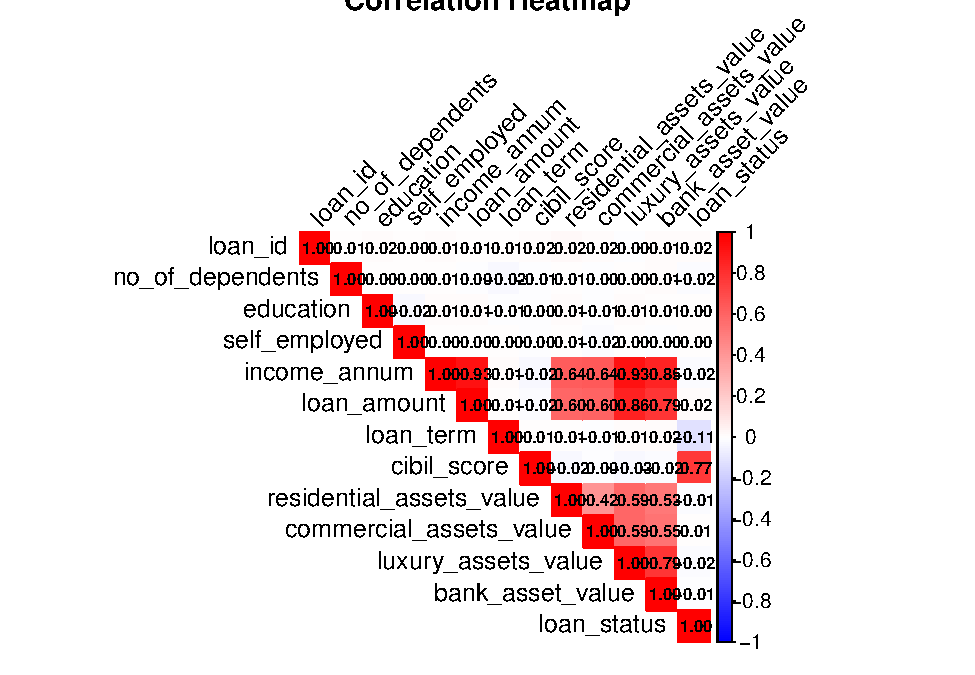
\includegraphics{Loan_approval_files/figure-latex/unnamed-chunk-13-1.pdf}

-The correlation analysis reveals key relationships between financial
factors and loan approval

-Strong positive correlations exist between loan amount and income,
luxury asset value and income, as well as bank asset value and income.

-Loan status has a high positive correlation with CIBIL score,
indicating that credit history significantly impacts loan approval.

-Moderate positive correlations are observed between various asset
values (residential, commercial, luxury) and loan amount.

-Loan status negatively correlates with bank, residential, and luxury
asset values, as well as income and number of dependents.

-Loan approval is not strongly influenced by factors like education or
commercial asset value.

-Applicants requesting longer loan terms tend to face more rejections,
suggesting that longer repayment periods decrease approval chances.

\begin{Shaded}
\begin{Highlighting}[]
\CommentTok{\#DISTRIBUTION OF THE DATASET EACH FEATURE}
\CommentTok{\# Load required libraries}
\FunctionTok{library}\NormalTok{(ggplot2)}
\FunctionTok{library}\NormalTok{(gridExtra)}




\CommentTok{\# Select numeric columns}
\NormalTok{numeric\_columns }\OtherTok{\textless{}{-}} \FunctionTok{names}\NormalTok{(loan\_data)[}\FunctionTok{sapply}\NormalTok{(loan\_data, is.numeric)]}

\CommentTok{\# Create empty list to store plots}
\NormalTok{plot\_list }\OtherTok{\textless{}{-}} \FunctionTok{list}\NormalTok{()}

\CommentTok{\# Create histogram with density curve for each numeric column}
\ControlFlowTok{for}\NormalTok{ (col }\ControlFlowTok{in}\NormalTok{ numeric\_columns) \{}
\NormalTok{  p }\OtherTok{\textless{}{-}} \FunctionTok{ggplot}\NormalTok{(loan\_data, }\FunctionTok{aes\_string}\NormalTok{(}\AttributeTok{x =}\NormalTok{ col)) }\SpecialCharTok{+}
    \FunctionTok{geom\_histogram}\NormalTok{(}\FunctionTok{aes}\NormalTok{(}\AttributeTok{y =} \FunctionTok{after\_stat}\NormalTok{(density)), }
                   \AttributeTok{bins =} \DecValTok{30}\NormalTok{, }
                   \AttributeTok{fill =} \StringTok{"skyblue"}\NormalTok{, }
                   \AttributeTok{color =} \StringTok{"black"}\NormalTok{, }
                   \AttributeTok{alpha =} \FloatTok{0.7}\NormalTok{) }\SpecialCharTok{+}
    \FunctionTok{geom\_density}\NormalTok{(}\AttributeTok{color =} \StringTok{"red"}\NormalTok{, }\AttributeTok{linewidth =} \DecValTok{1}\NormalTok{) }\SpecialCharTok{+}
    \FunctionTok{ggtitle}\NormalTok{(col) }\SpecialCharTok{+}
    \FunctionTok{theme\_minimal}\NormalTok{() }\SpecialCharTok{+}
    \FunctionTok{theme}\NormalTok{(}\AttributeTok{axis.title.x =} \FunctionTok{element\_blank}\NormalTok{())}
  
\NormalTok{  plot\_list[[col]] }\OtherTok{\textless{}{-}}\NormalTok{ p}
\NormalTok{\}}

\CommentTok{\# Calculate grid dimensions (4x4 layout or whatever fits the number of columns)}
\NormalTok{n\_plots }\OtherTok{\textless{}{-}} \FunctionTok{length}\NormalTok{(plot\_list)}
\NormalTok{n\_rows }\OtherTok{\textless{}{-}} \FunctionTok{ceiling}\NormalTok{(}\FunctionTok{sqrt}\NormalTok{(n\_plots))}
\NormalTok{n\_cols }\OtherTok{\textless{}{-}} \FunctionTok{ceiling}\NormalTok{(n\_plots }\SpecialCharTok{/}\NormalTok{ n\_rows)}

\CommentTok{\# Arrange plots in a grid and display}
\FunctionTok{grid.arrange}\NormalTok{(}\AttributeTok{grobs =}\NormalTok{ plot\_list, }\AttributeTok{nrow =} \DecValTok{4}\NormalTok{, }\AttributeTok{ncol =} \DecValTok{4}\NormalTok{)}
\end{Highlighting}
\end{Shaded}

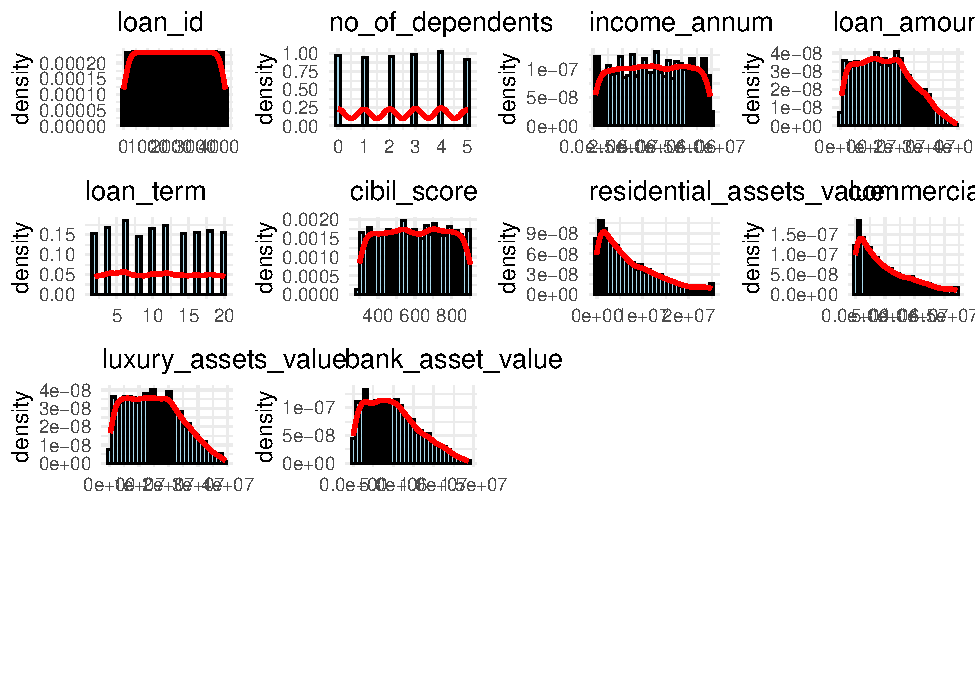
\includegraphics{Loan_approval_files/figure-latex/unnamed-chunk-14-1.pdf}

There are more applicants in the dataset they are either renting or
living in other people space -More applicants are Approved in the
dataset -There are more applicants having 4 no of dependents and less
with 0 - 3 and 5 -Income annum majority lies b/w 0.4 and 0.6 -majority
is in loan amount 1.1 -there are more applicants with loan term of 6
years -many applicants donot have any commercial asset -majority luxury
asset value is 1.5 -More applicants have the bank asset value of 0.1
-dataset have almost equal educated and uneducated / self - employed and
not self emplyed applicants

\begin{Shaded}
\begin{Highlighting}[]
\CommentTok{\# \% of Graduate and Ungraduate Applicants in dataset}

\CommentTok{\# Load required libraries}
\FunctionTok{library}\NormalTok{(ggplot2)}


\CommentTok{\# Count the frequency of each education category}
\NormalTok{education\_counts }\OtherTok{\textless{}{-}} \FunctionTok{table}\NormalTok{(loan\_data}\SpecialCharTok{$}\NormalTok{education)}
\NormalTok{education\_df }\OtherTok{\textless{}{-}} \FunctionTok{as.data.frame}\NormalTok{(education\_counts)}
\FunctionTok{names}\NormalTok{(education\_df) }\OtherTok{\textless{}{-}} \FunctionTok{c}\NormalTok{(}\StringTok{"education"}\NormalTok{, }\StringTok{"count"}\NormalTok{)}

\CommentTok{\# Create the pie chart}

\FunctionTok{ggplot}\NormalTok{(education\_df, }\FunctionTok{aes}\NormalTok{(}\AttributeTok{x =} \StringTok{""}\NormalTok{, }\AttributeTok{y =}\NormalTok{ count, }\AttributeTok{fill =}\NormalTok{ education)) }\SpecialCharTok{+}
  \FunctionTok{geom\_bar}\NormalTok{(}\AttributeTok{stat =} \StringTok{"identity"}\NormalTok{, }\AttributeTok{width =} \DecValTok{1}\NormalTok{) }\SpecialCharTok{+}
  \FunctionTok{coord\_polar}\NormalTok{(}\StringTok{"y"}\NormalTok{, }\AttributeTok{start =} \DecValTok{0}\NormalTok{) }\SpecialCharTok{+}
  \CommentTok{\# Add percentage labels}
  \FunctionTok{geom\_text}\NormalTok{(}\FunctionTok{aes}\NormalTok{(}\AttributeTok{label =} \FunctionTok{paste0}\NormalTok{(}\FunctionTok{round}\NormalTok{(count}\SpecialCharTok{/}\FunctionTok{sum}\NormalTok{(count)}\SpecialCharTok{*}\DecValTok{100}\NormalTok{, }\DecValTok{1}\NormalTok{), }\StringTok{"\%"}\NormalTok{)),}
            \AttributeTok{position =} \FunctionTok{position\_stack}\NormalTok{(}\AttributeTok{vjust =} \FloatTok{0.5}\NormalTok{)) }\SpecialCharTok{+}
  \CommentTok{\# Custom colors similar to Plotly T10}
  \FunctionTok{scale\_fill\_manual}\NormalTok{(}\AttributeTok{values =} \FunctionTok{c}\NormalTok{(}\StringTok{"\#4C78A8"}\NormalTok{, }\StringTok{"\#F58518"}\NormalTok{)) }\SpecialCharTok{+}
  \CommentTok{\# Customize appearance}
  
  \FunctionTok{labs}\NormalTok{(}\AttributeTok{title =} \StringTok{"\% of Graduate and Ungraduate Applicants in dataset"}\NormalTok{,}
       \AttributeTok{x =} \ConstantTok{NULL}\NormalTok{, }\AttributeTok{y =} \ConstantTok{NULL}\NormalTok{, }\AttributeTok{fill =} \StringTok{"Education"}\NormalTok{) }\SpecialCharTok{+}
  \FunctionTok{theme\_minimal}\NormalTok{() }\SpecialCharTok{+}
  \FunctionTok{theme}\NormalTok{(}\AttributeTok{axis.text =} \FunctionTok{element\_blank}\NormalTok{(),}
        \AttributeTok{axis.ticks =} \FunctionTok{element\_blank}\NormalTok{(),}
        \AttributeTok{panel.grid =} \FunctionTok{element\_blank}\NormalTok{())}
\end{Highlighting}
\end{Shaded}

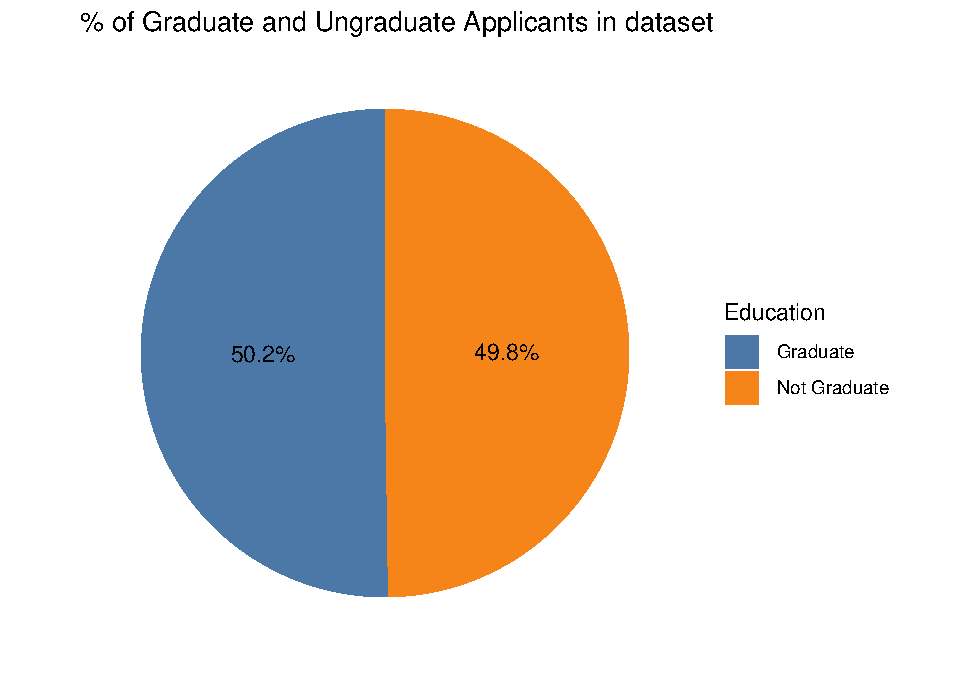
\includegraphics{Loan_approval_files/figure-latex/unnamed-chunk-15-1.pdf}

\begin{Shaded}
\begin{Highlighting}[]
\CommentTok{\# \% of self\_employed people and rejection in dataset}

\CommentTok{\# Load necessary library}
\FunctionTok{library}\NormalTok{(ggplot2)}

\CommentTok{\# Assuming loan\_data is your data frame}
\CommentTok{\# Summarize the data to get counts for each self\_employed status}
\NormalTok{self\_employed\_counts }\OtherTok{\textless{}{-}} \FunctionTok{aggregate}\NormalTok{(loan\_id }\SpecialCharTok{\textasciitilde{}}\NormalTok{ self\_employed, }\AttributeTok{data =}\NormalTok{ loan\_data, }\AttributeTok{FUN =}\NormalTok{ length)}

\CommentTok{\# Calculate the percentage for each self\_employed status}
\NormalTok{self\_employed\_counts}\SpecialCharTok{$}\NormalTok{percentage }\OtherTok{\textless{}{-}}\NormalTok{ self\_employed\_counts}\SpecialCharTok{$}\NormalTok{loan\_id }\SpecialCharTok{/} \FunctionTok{sum}\NormalTok{(self\_employed\_counts}\SpecialCharTok{$}\NormalTok{loan\_id) }\SpecialCharTok{*} \DecValTok{100}

\CommentTok{\# Create the pie chart with percentage labels}
\FunctionTok{ggplot}\NormalTok{(self\_employed\_counts, }\FunctionTok{aes}\NormalTok{(}\AttributeTok{x =} \StringTok{""}\NormalTok{, }\AttributeTok{y =}\NormalTok{ loan\_id, }\AttributeTok{fill =}\NormalTok{ self\_employed)) }\SpecialCharTok{+}
  \FunctionTok{geom\_bar}\NormalTok{(}\AttributeTok{stat =} \StringTok{"identity"}\NormalTok{, }\AttributeTok{width =} \DecValTok{1}\NormalTok{) }\SpecialCharTok{+}
  \FunctionTok{coord\_polar}\NormalTok{(}\AttributeTok{theta =} \StringTok{"y"}\NormalTok{) }\SpecialCharTok{+}
  \FunctionTok{labs}\NormalTok{(}\AttributeTok{title =} \StringTok{"\% of Self{-}Employed People and Rejection in Dataset"}\NormalTok{) }\SpecialCharTok{+}
  \FunctionTok{theme\_void}\NormalTok{() }\SpecialCharTok{+}
  \FunctionTok{scale\_fill\_manual}\NormalTok{(}\AttributeTok{values =} \FunctionTok{c}\NormalTok{(}\StringTok{"\#1f77b4"}\NormalTok{, }\StringTok{"\#ff7f0e"}\NormalTok{, }\StringTok{"\#2ca02c"}\NormalTok{, }\StringTok{"\#d62728"}\NormalTok{, }\StringTok{"\#9467bd"}\NormalTok{, }\StringTok{"\#8c564b"}\NormalTok{, }\StringTok{"\#e377c2"}\NormalTok{, }\StringTok{"\#7f7f7f"}\NormalTok{, }\StringTok{"\#bcbd22"}\NormalTok{, }\StringTok{"\#17becf"}\NormalTok{)) }\SpecialCharTok{+}
  \FunctionTok{geom\_text}\NormalTok{(}\FunctionTok{aes}\NormalTok{(}\AttributeTok{label =} \FunctionTok{paste0}\NormalTok{(}\FunctionTok{round}\NormalTok{(percentage, }\DecValTok{1}\NormalTok{), }\StringTok{"\%"}\NormalTok{)), }
            \AttributeTok{position =} \FunctionTok{position\_stack}\NormalTok{(}\AttributeTok{vjust =} \FloatTok{0.5}\NormalTok{))}
\end{Highlighting}
\end{Shaded}

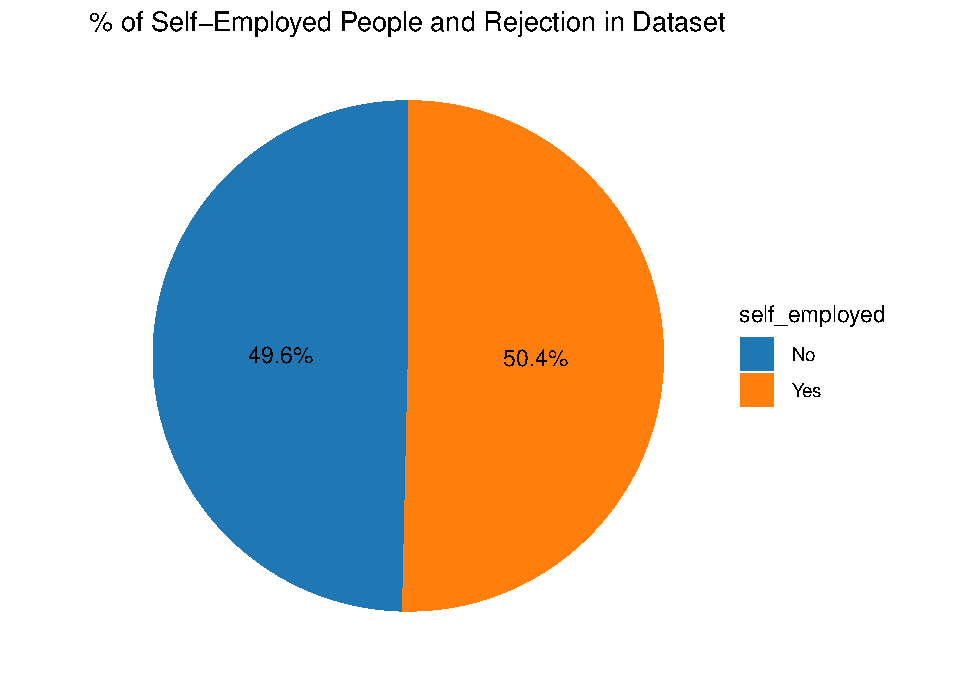
\includegraphics{Loan_approval_files/figure-latex/unnamed-chunk-16-1.pdf}

\begin{Shaded}
\begin{Highlighting}[]
\CommentTok{\# \% Approval and Rejection in Dataset}

\CommentTok{\# Load necessary library}
\FunctionTok{library}\NormalTok{(ggplot2)}

\CommentTok{\# Assuming loan\_data is your data frame}
\CommentTok{\# Summarize the data to get counts for each loan\_status}
\NormalTok{loan\_status\_counts }\OtherTok{\textless{}{-}} \FunctionTok{aggregate}\NormalTok{(loan\_id }\SpecialCharTok{\textasciitilde{}}\NormalTok{ loan\_status, }\AttributeTok{data =}\NormalTok{ loan\_data, }\AttributeTok{FUN =}\NormalTok{ length)}

\CommentTok{\# Calculate the percentage for each loan\_status}
\NormalTok{loan\_status\_counts}\SpecialCharTok{$}\NormalTok{percentage }\OtherTok{\textless{}{-}}\NormalTok{ loan\_status\_counts}\SpecialCharTok{$}\NormalTok{loan\_id }\SpecialCharTok{/} \FunctionTok{sum}\NormalTok{(loan\_status\_counts}\SpecialCharTok{$}\NormalTok{loan\_id) }\SpecialCharTok{*} \DecValTok{100}

\CommentTok{\# Create the pie chart with percentage labels}
\FunctionTok{ggplot}\NormalTok{(loan\_status\_counts, }\FunctionTok{aes}\NormalTok{(}\AttributeTok{x =} \StringTok{""}\NormalTok{, }\AttributeTok{y =}\NormalTok{ loan\_id, }\AttributeTok{fill =}\NormalTok{ loan\_status)) }\SpecialCharTok{+}
  \FunctionTok{geom\_bar}\NormalTok{(}\AttributeTok{stat =} \StringTok{"identity"}\NormalTok{, }\AttributeTok{width =} \DecValTok{1}\NormalTok{) }\SpecialCharTok{+}
  \FunctionTok{coord\_polar}\NormalTok{(}\AttributeTok{theta =} \StringTok{"y"}\NormalTok{) }\SpecialCharTok{+}
  \FunctionTok{labs}\NormalTok{(}\AttributeTok{title =} \StringTok{"\% of Approval and Rejection in Dataset"}\NormalTok{) }\SpecialCharTok{+}
  \FunctionTok{theme\_void}\NormalTok{() }\SpecialCharTok{+}
  \FunctionTok{scale\_fill\_manual}\NormalTok{(}\AttributeTok{values =} \FunctionTok{c}\NormalTok{(}\StringTok{"\#1f77b4"}\NormalTok{, }\StringTok{"\#ff7f0e"}\NormalTok{, }\StringTok{"\#2ca02c"}\NormalTok{, }\StringTok{"\#d62728"}\NormalTok{, }\StringTok{"\#9467bd"}\NormalTok{, }\StringTok{"\#8c564b"}\NormalTok{, }\StringTok{"\#e377c2"}\NormalTok{, }\StringTok{"\#7f7f7f"}\NormalTok{, }\StringTok{"\#bcbd22"}\NormalTok{, }\StringTok{"\#17becf"}\NormalTok{)) }\SpecialCharTok{+}
  \FunctionTok{geom\_text}\NormalTok{(}\FunctionTok{aes}\NormalTok{(}\AttributeTok{label =} \FunctionTok{paste0}\NormalTok{(}\FunctionTok{round}\NormalTok{(percentage, }\DecValTok{1}\NormalTok{), }\StringTok{"\%"}\NormalTok{)), }
            \AttributeTok{position =} \FunctionTok{position\_stack}\NormalTok{(}\AttributeTok{vjust =} \FloatTok{0.5}\NormalTok{))}
\end{Highlighting}
\end{Shaded}

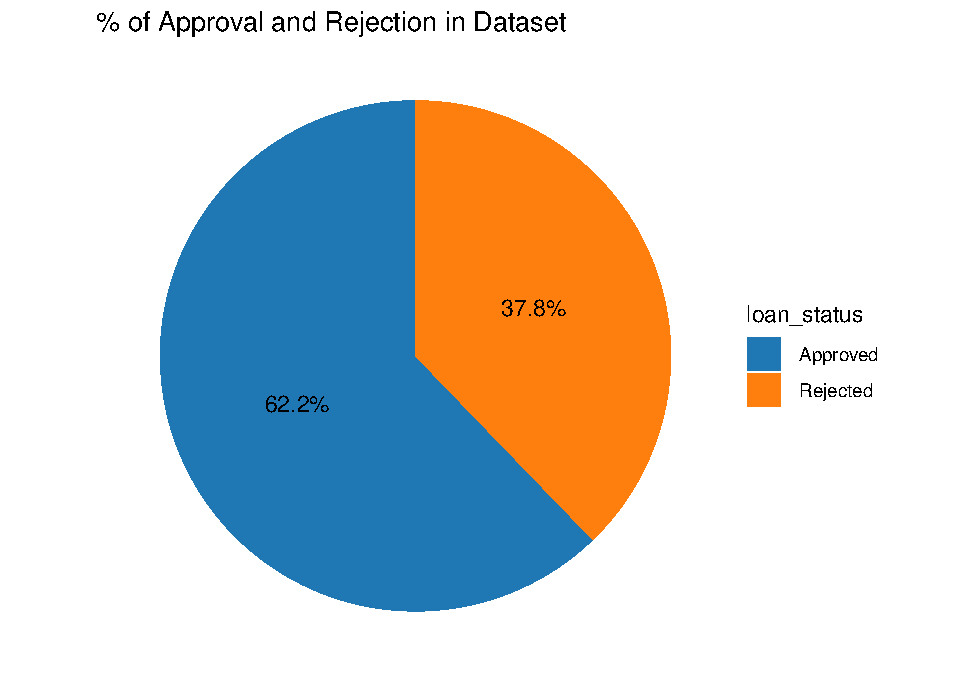
\includegraphics{Loan_approval_files/figure-latex/unnamed-chunk-17-1.pdf}

-sample has slightly more educated Applicants , and slightly more
self\_employed Applicants -dataset have more Approved loan status then
Rejected

\section{Visualizing NUMERIC FEATURES
RELATIONSHIP(CORRELATION)}\label{visualizing-numeric-features-relationshipcorrelation}

\begin{Shaded}
\begin{Highlighting}[]
\CommentTok{\# Load necessary library}
\FunctionTok{library}\NormalTok{(ggplot2)}

\CommentTok{\# Define custom label functions for the axes}
\NormalTok{custom\_labels }\OtherTok{\textless{}{-}} \ControlFlowTok{function}\NormalTok{(x) }\FunctionTok{sprintf}\NormalTok{(}\StringTok{"\%.1f"}\NormalTok{, x }\SpecialCharTok{/} \FloatTok{1e7}\NormalTok{)}

\CommentTok{\# Create the scatter plot}
\FunctionTok{ggplot}\NormalTok{(loan\_data, }\FunctionTok{aes}\NormalTok{(}\AttributeTok{x =}\NormalTok{ income\_annum, }\AttributeTok{y =}\NormalTok{ loan\_amount, }\AttributeTok{color =}\NormalTok{ loan\_status)) }\SpecialCharTok{+}
  \FunctionTok{geom\_point}\NormalTok{() }\SpecialCharTok{+}
  \FunctionTok{labs}\NormalTok{(}
    \AttributeTok{x =} \StringTok{"Annual Income (in e7)"}\NormalTok{,}
    \AttributeTok{y =} \StringTok{"Loan Amount (in e7)"}\NormalTok{,}
    \AttributeTok{title =} \StringTok{"Loan Amount vs Income by Loan Status"}
\NormalTok{  ) }\SpecialCharTok{+}
  \FunctionTok{theme\_minimal}\NormalTok{() }\SpecialCharTok{+}
  \FunctionTok{theme}\NormalTok{(}\AttributeTok{plot.title =} \FunctionTok{element\_text}\NormalTok{(}\AttributeTok{hjust =} \FloatTok{0.5}\NormalTok{)) }\SpecialCharTok{+}
  \FunctionTok{scale\_color\_manual}\NormalTok{(}\AttributeTok{values =} \FunctionTok{c}\NormalTok{(}\StringTok{"blue"}\NormalTok{, }\StringTok{"orange"}\NormalTok{, }\StringTok{"green"}\NormalTok{, }\StringTok{"red"}\NormalTok{, }\StringTok{"purple"}\NormalTok{, }\StringTok{"brown"}\NormalTok{, }\StringTok{"pink"}\NormalTok{, }\StringTok{"gray"}\NormalTok{, }\StringTok{"yellow"}\NormalTok{, }\StringTok{"cyan"}\NormalTok{)) }\SpecialCharTok{+}
  \FunctionTok{scale\_x\_continuous}\NormalTok{(}\AttributeTok{labels =}\NormalTok{ custom\_labels) }\SpecialCharTok{+}
  \FunctionTok{scale\_y\_continuous}\NormalTok{(}\AttributeTok{labels =}\NormalTok{ custom\_labels)}
\end{Highlighting}
\end{Shaded}

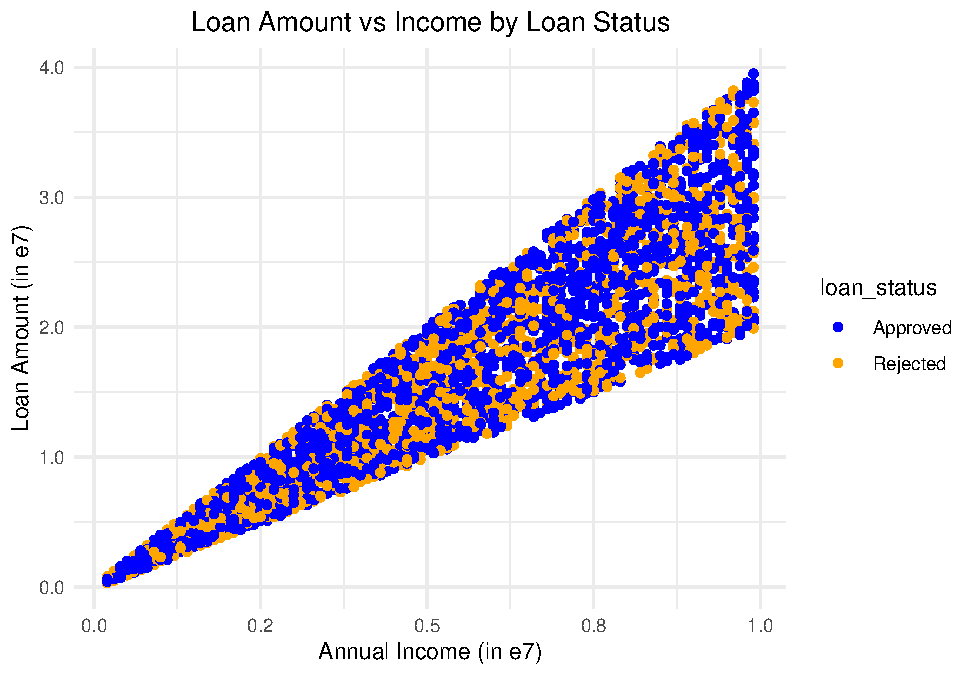
\includegraphics{Loan_approval_files/figure-latex/unnamed-chunk-18-1.pdf}
-Applicants with high income tends to take apply for high loan amounts

-Loan Amount vs Bank Balance by Loan Status

\begin{Shaded}
\begin{Highlighting}[]
\CommentTok{\# Load necessary library}
\FunctionTok{library}\NormalTok{(ggplot2)}

\CommentTok{\# Scale the data by dividing by 10\^{}7}
\NormalTok{loan\_data\_scaled }\OtherTok{\textless{}{-}}\NormalTok{ loan\_data}
\NormalTok{loan\_data\_scaled}\SpecialCharTok{$}\NormalTok{bank\_asset\_value\_scaled }\OtherTok{\textless{}{-}}\NormalTok{ loan\_data\_scaled}\SpecialCharTok{$}\NormalTok{bank\_asset\_value }\SpecialCharTok{/} \FloatTok{1e7}
\NormalTok{loan\_data\_scaled}\SpecialCharTok{$}\NormalTok{luxury\_assets\_value\_scaled }\OtherTok{\textless{}{-}}\NormalTok{ loan\_data\_scaled}\SpecialCharTok{$}\NormalTok{luxury\_assets\_value }\SpecialCharTok{/} \FloatTok{1e7}

\CommentTok{\# Create the scatter plot}
\FunctionTok{ggplot}\NormalTok{(loan\_data\_scaled, }\FunctionTok{aes}\NormalTok{(}\AttributeTok{x =}\NormalTok{ bank\_asset\_value\_scaled, }\AttributeTok{y =}\NormalTok{ luxury\_assets\_value\_scaled, }\AttributeTok{color =}\NormalTok{ loan\_status)) }\SpecialCharTok{+}
  \FunctionTok{geom\_point}\NormalTok{() }\SpecialCharTok{+}
  \FunctionTok{labs}\NormalTok{(}
    \AttributeTok{x =} \StringTok{"Bank Balance (in 10\^{}7)"}\NormalTok{,}
    \AttributeTok{y =} \StringTok{"Luxuries (in 10\^{}7)"}\NormalTok{,}
    \AttributeTok{title =} \StringTok{"Loan Amount vs Bank Balance by Loan Status"}
\NormalTok{  ) }\SpecialCharTok{+}
  \FunctionTok{theme\_minimal}\NormalTok{() }\SpecialCharTok{+}
  \FunctionTok{theme}\NormalTok{(}\AttributeTok{plot.title =} \FunctionTok{element\_text}\NormalTok{(}\AttributeTok{hjust =} \FloatTok{0.5}\NormalTok{)) }\SpecialCharTok{+}
  \FunctionTok{scale\_color\_manual}\NormalTok{(}\AttributeTok{values =} \FunctionTok{c}\NormalTok{(}\StringTok{"blue"}\NormalTok{, }\StringTok{"orange"}\NormalTok{, }\StringTok{"green"}\NormalTok{, }\StringTok{"red"}\NormalTok{, }\StringTok{"purple"}\NormalTok{, }\StringTok{"brown"}\NormalTok{, }\StringTok{"pink"}\NormalTok{, }\StringTok{"gray"}\NormalTok{, }\StringTok{"yellow"}\NormalTok{, }\StringTok{"cyan"}\NormalTok{)) }\SpecialCharTok{+}
  \FunctionTok{scale\_x\_continuous}\NormalTok{(}\AttributeTok{labels =}\NormalTok{ custom\_labels) }\SpecialCharTok{+}
  \FunctionTok{scale\_y\_continuous}\NormalTok{(}\AttributeTok{labels =}\NormalTok{ custom\_labels)}
\end{Highlighting}
\end{Shaded}

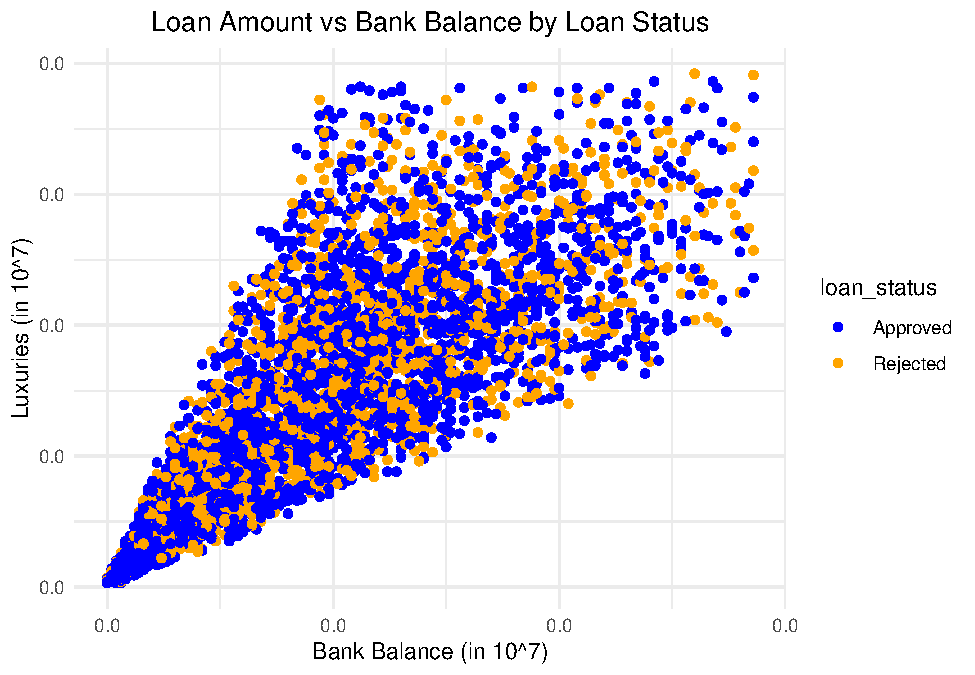
\includegraphics{Loan_approval_files/figure-latex/unnamed-chunk-19-1.pdf}
-Applicants with more balance in their accounts tend to buy high value
luxury items

\begin{Shaded}
\begin{Highlighting}[]
\CommentTok{\# Load necessary libraries}
\FunctionTok{library}\NormalTok{(GGally)}
\FunctionTok{library}\NormalTok{(ggplot2)}

\CommentTok{\# Scale the data by dividing by 10\^{}7}
\NormalTok{loan\_data\_scaled}\SpecialCharTok{$}\NormalTok{income\_annum\_scaled }\OtherTok{\textless{}{-}}\NormalTok{ loan\_data\_scaled}\SpecialCharTok{$}\NormalTok{income\_annum }\SpecialCharTok{/} \FloatTok{1e7}
\NormalTok{loan\_data\_scaled}\SpecialCharTok{$}\NormalTok{loan\_amount\_scaled }\OtherTok{\textless{}{-}}\NormalTok{ loan\_data\_scaled}\SpecialCharTok{$}\NormalTok{loan\_amount }\SpecialCharTok{/} \FloatTok{1e7}
\NormalTok{loan\_data\_scaled}\SpecialCharTok{$}\NormalTok{cibil\_score\_scaled }\OtherTok{\textless{}{-}}\NormalTok{ loan\_data\_scaled}\SpecialCharTok{$}\NormalTok{cibil\_score }\SpecialCharTok{/} \FloatTok{1e7}

\CommentTok{\# Create the pair plot}
\FunctionTok{ggpairs}\NormalTok{(}
\NormalTok{  loan\_data\_scaled, }
  \AttributeTok{columns =} \FunctionTok{c}\NormalTok{(}\StringTok{\textquotesingle{}income\_annum\_scaled\textquotesingle{}}\NormalTok{, }\StringTok{\textquotesingle{}loan\_amount\_scaled\textquotesingle{}}\NormalTok{, }\StringTok{\textquotesingle{}cibil\_score\_scaled\textquotesingle{}}\NormalTok{), }
  \FunctionTok{aes}\NormalTok{(}\AttributeTok{color =}\NormalTok{ loan\_status),}
  \AttributeTok{columnLabels =} \FunctionTok{c}\NormalTok{(}\StringTok{\textquotesingle{}Income (in 10\^{}7)\textquotesingle{}}\NormalTok{, }\StringTok{\textquotesingle{}Loan Amount (in 10\^{}7)\textquotesingle{}}\NormalTok{, }\StringTok{\textquotesingle{}CIBIL Score (in 10\^{}7)\textquotesingle{}}\NormalTok{)}
\NormalTok{) }\SpecialCharTok{+}
  \FunctionTok{theme\_minimal}\NormalTok{()}
\end{Highlighting}
\end{Shaded}

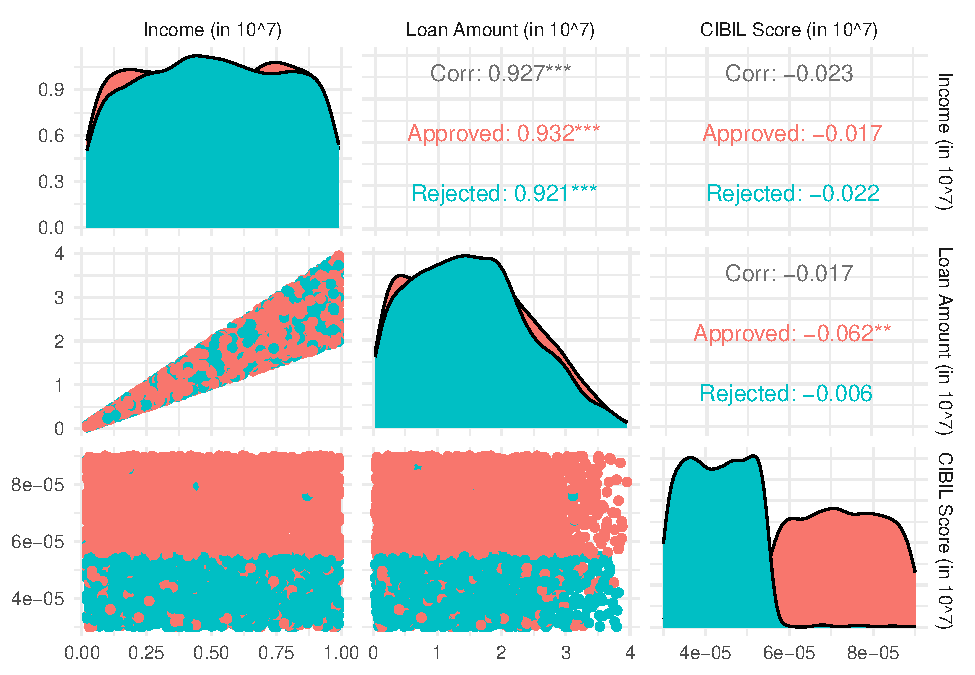
\includegraphics{Loan_approval_files/figure-latex/unnamed-chunk-20-1.pdf}
-No relation between cibil score and income annum and loan amount

\begin{Shaded}
\begin{Highlighting}[]
\CommentTok{\# ANALYZING THE FEATURE HAVING THE HIGH CHANCE OF LOAN APPROVAL}
\CommentTok{\# Load necessary libraries}
\FunctionTok{library}\NormalTok{(ggplot2)}
\FunctionTok{library}\NormalTok{(gridExtra)}

\CommentTok{\# Select numeric columns}
\NormalTok{numeric\_columns }\OtherTok{\textless{}{-}} \FunctionTok{sapply}\NormalTok{(loan\_data, is.numeric)}
\NormalTok{numeric\_data }\OtherTok{\textless{}{-}}\NormalTok{ loan\_data[, numeric\_columns]}

\CommentTok{\# Scale the numeric data by dividing by 10\^{}7}
\NormalTok{scaled\_data }\OtherTok{\textless{}{-}} \FunctionTok{as.data.frame}\NormalTok{(}\FunctionTok{lapply}\NormalTok{(numeric\_data, }\ControlFlowTok{function}\NormalTok{(x) x }\SpecialCharTok{/} \FloatTok{1e7}\NormalTok{))}

\CommentTok{\# Add the loan\_status column back to the scaled data}
\NormalTok{scaled\_data}\SpecialCharTok{$}\NormalTok{loan\_status }\OtherTok{\textless{}{-}}\NormalTok{ loan\_data}\SpecialCharTok{$}\NormalTok{loan\_status}

\CommentTok{\# Create a list to store the plots}
\NormalTok{plots }\OtherTok{\textless{}{-}} \FunctionTok{list}\NormalTok{()}

\CommentTok{\# Create histograms for each numeric column}
\ControlFlowTok{for}\NormalTok{ (column }\ControlFlowTok{in} \FunctionTok{names}\NormalTok{(scaled\_data)[}\SpecialCharTok{{-}}\FunctionTok{ncol}\NormalTok{(scaled\_data)]) \{}
\NormalTok{  p }\OtherTok{\textless{}{-}} \FunctionTok{ggplot}\NormalTok{(scaled\_data, }\FunctionTok{aes\_string}\NormalTok{(}\AttributeTok{x =}\NormalTok{ column, }\AttributeTok{fill =} \StringTok{"loan\_status"}\NormalTok{)) }\SpecialCharTok{+}
    \FunctionTok{geom\_histogram}\NormalTok{(}\AttributeTok{bins =} \DecValTok{30}\NormalTok{, }\AttributeTok{alpha =} \FloatTok{0.7}\NormalTok{, }\AttributeTok{position =} \StringTok{"identity"}\NormalTok{) }\SpecialCharTok{+}
    \FunctionTok{geom\_density}\NormalTok{(}\AttributeTok{alpha =} \FloatTok{0.3}\NormalTok{) }\SpecialCharTok{+}
    \FunctionTok{labs}\NormalTok{(}\AttributeTok{title =}\NormalTok{ column, }\AttributeTok{x =} \FunctionTok{paste}\NormalTok{(column, }\StringTok{"(in 10\^{}7)"}\NormalTok{), }\AttributeTok{y =} \StringTok{"Frequency"}\NormalTok{) }\SpecialCharTok{+}
    \FunctionTok{theme\_minimal}\NormalTok{()}
\NormalTok{  plots[[column]] }\OtherTok{\textless{}{-}}\NormalTok{ p}
\NormalTok{\}}

\CommentTok{\# Arrange the plots in a grid}
\FunctionTok{grid.arrange}\NormalTok{(}\AttributeTok{grobs =}\NormalTok{ plots, }\AttributeTok{ncol =} \DecValTok{4}\NormalTok{)}
\end{Highlighting}
\end{Shaded}

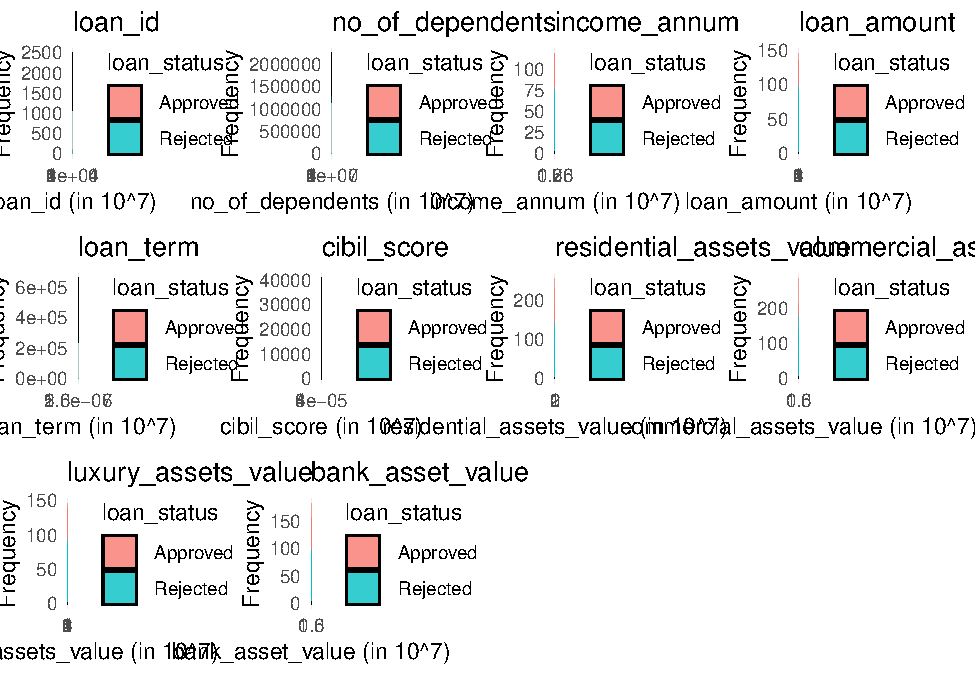
\includegraphics{Loan_approval_files/figure-latex/unnamed-chunk-21-1.pdf}

\begin{itemize}
\tightlist
\item
  As the cibil\_score increases the Approval of loan status has been
  seen
\item
  INDICATING applicants having a good credit history and loan replayment
  tends to have higher chances of loan approval
\end{itemize}

\section{MODELLING}\label{modelling}

\begin{Shaded}
\begin{Highlighting}[]
\CommentTok{\# Feature Selection}

\CommentTok{\# Load necessary libraries}
\FunctionTok{library}\NormalTok{(dplyr)}

\CommentTok{\# Drop unnecessary columns}
\CommentTok{\# Drop \textquotesingle{}loan\_id\textquotesingle{} column {-} Not needed for analysis}
\NormalTok{loan\_data }\OtherTok{\textless{}{-}}\NormalTok{ loan\_data }\SpecialCharTok{\%\textgreater{}\%} \FunctionTok{select}\NormalTok{(}\SpecialCharTok{{-}}\NormalTok{loan\_id)}
\end{Highlighting}
\end{Shaded}

\#Checking Class Imbalance

\begin{Shaded}
\begin{Highlighting}[]
\CommentTok{\# Class distribution}
\CommentTok{\# ggplot(loan\_data, aes(x=factor(loan\_status), fill=factor(loan\_status))) + }
\CommentTok{\#   geom\_bar(alpha=0.7) + }
\CommentTok{\#   theme\_minimal() +}
\CommentTok{\#   ggtitle("Loan Approval Distribution") +}
\CommentTok{\#   scale\_fill\_manual(values = c("red", "green"), labels = c("Rejected", "Approved")) +}
\CommentTok{\#   labs(x = "Loan Status", fill = "Status")}
\end{Highlighting}
\end{Shaded}

\#KNN can be affected by imbalance because it tends to favor the
majority class. \#This means the model might predict 0 (Rejected) too
often, leading to \#poor recall for 1 (Approved).

\begin{Shaded}
\begin{Highlighting}[]
\CommentTok{\# library(themis)}
\CommentTok{\# library(recipes)}
\CommentTok{\# }
\CommentTok{\# \# Apply SMOTE using recipes (tidymodels framework)}
\CommentTok{\# loan\_data$education \textless{}{-} as.integer(factor(loan\_data$education))}
\CommentTok{\# loan\_data$self\_employed \textless{}{-} as.integer(factor(loan\_data$self\_employed))}
\CommentTok{\# }
\CommentTok{\# \# Now apply SMOTE}
\CommentTok{\# rec \textless{}{-} recipe(loan\_status \textasciitilde{} ., data = loan\_data) \%\textgreater{}\%}
\CommentTok{\#   step\_smote(loan\_status, over\_ratio = 1) \%\textgreater{}\%}
\CommentTok{\#   prep() \%\textgreater{}\%}
\CommentTok{\#   bake(new\_data = NULL)}
\CommentTok{\# }
\CommentTok{\# table(rec$loan\_status)}
\CommentTok{\# }
\CommentTok{\# loan\_data \textless{}{-} rec}
\end{Highlighting}
\end{Shaded}

\#Verify Balance

\begin{Shaded}
\begin{Highlighting}[]
\CommentTok{\# ggplot(loan\_data, aes(x = factor(loan\_status), fill = factor(loan\_status))) +}
\CommentTok{\#   geom\_bar(alpha = 0.7) +}
\CommentTok{\#   theme\_minimal() +}
\CommentTok{\#   ggtitle("Loan Approval Distribution After SMOTE") +}
\CommentTok{\#   scale\_fill\_manual(values = c("red", "green"), labels = c("Rejected", "Approved")) +}
\CommentTok{\#   labs(x = "Loan Status", fill = "Status")}
\end{Highlighting}
\end{Shaded}

\begin{Shaded}
\begin{Highlighting}[]
\CommentTok{\#Convert Categorical Variables {-} Since KNN works best with numerical data, convert categorical variables into factors.}

\NormalTok{loan\_data}\SpecialCharTok{$}\NormalTok{education }\OtherTok{\textless{}{-}} \FunctionTok{as.factor}\NormalTok{(loan\_data}\SpecialCharTok{$}\NormalTok{education)}

\NormalTok{loan\_data}\SpecialCharTok{$}\NormalTok{self\_employed }\OtherTok{\textless{}{-}} \FunctionTok{as.factor}\NormalTok{(loan\_data}\SpecialCharTok{$}\NormalTok{self\_employed)}
\end{Highlighting}
\end{Shaded}

\begin{Shaded}
\begin{Highlighting}[]
\CommentTok{\#Normalize Numerical Features}

\CommentTok{\#Formula}
\NormalTok{normalize }\OtherTok{\textless{}{-}} \ControlFlowTok{function}\NormalTok{(x) \{}
  \FunctionTok{return}\NormalTok{((x }\SpecialCharTok{{-}} \FunctionTok{min}\NormalTok{(x)) }\SpecialCharTok{/}\NormalTok{ (}\FunctionTok{max}\NormalTok{(x) }\SpecialCharTok{{-}} \FunctionTok{min}\NormalTok{(x)))}
\NormalTok{\}}

\CommentTok{\# Normalize relevant numerical columns}
\NormalTok{loan\_data[, }\FunctionTok{c}\NormalTok{(}\StringTok{"no\_of\_dependents"}\NormalTok{, }\StringTok{"income\_annum"}\NormalTok{, }\StringTok{"loan\_amount"}\NormalTok{, }\StringTok{"loan\_term"}\NormalTok{, }
              \StringTok{"cibil\_score"}\NormalTok{, }\StringTok{"residential\_assets\_value"}\NormalTok{, }\StringTok{"commercial\_assets\_value"}\NormalTok{, }\StringTok{"luxury\_assets\_value"}\NormalTok{, }\StringTok{"bank\_asset\_value"}\NormalTok{)] }\OtherTok{\textless{}{-}} 
  \FunctionTok{apply}\NormalTok{(loan\_data[, }\FunctionTok{c}\NormalTok{(}\StringTok{"no\_of\_dependents"}\NormalTok{, }\StringTok{"income\_annum"}\NormalTok{, }\StringTok{"loan\_amount"}\NormalTok{, }\StringTok{"loan\_term"}\NormalTok{, }
                      \StringTok{"cibil\_score"}\NormalTok{, }\StringTok{"residential\_assets\_value"}\NormalTok{, }\StringTok{"commercial\_assets\_value"}\NormalTok{, }\StringTok{"luxury\_assets\_value"}\NormalTok{, }\StringTok{"bank\_asset\_value"}\NormalTok{)], }
        \DecValTok{2}\NormalTok{, normalize)}

\CommentTok{\#Show first rows}
\FunctionTok{head}\NormalTok{(loan\_data)}
\end{Highlighting}
\end{Shaded}

\begin{verbatim}
##   no_of_dependents     education self_employed income_annum loan_amount
## 1              0.4      Graduate            No    0.9690722   0.7551020
## 2              0.0  Not Graduate           Yes    0.4020619   0.3035714
## 3              0.6      Graduate            No    0.9175258   0.7500000
## 4              0.6      Graduate            No    0.8247423   0.7755102
## 5              1.0  Not Graduate           Yes    0.9896907   0.6096939
## 6              0.0      Graduate           Yes    0.4742268   0.3367347
##   loan_term cibil_score residential_assets_value commercial_assets_value
## 1 0.5555556  0.79666667                0.0998004               1.0000000
## 2 0.3333333  0.19500000                0.1117764               0.1290323
## 3 1.0000000  0.34333333                0.2874251               0.2639296
## 4 0.3333333  0.27833333                0.7305389               0.1935484
## 5 1.0000000  0.13666667                0.4990020               0.4809384
## 6 0.4444444  0.03166667                0.2754491               0.4868035
##   luxury_assets_value bank_asset_value loan_status
## 1           0.5758355        0.5594406    Approved
## 2           0.2185090        0.2307692    Rejected
## 3           0.8483290        0.8951049    Rejected
## 4           0.5912596        0.5524476    Rejected
## 5           0.7480720        0.3496503    Rejected
## 6           0.3444730        0.3566434    Rejected
\end{verbatim}

\#Training the KNN Model \#Split Data into Training \& Testing Sets
\#Using Hold Out Estimation

\begin{Shaded}
\begin{Highlighting}[]
\CommentTok{\# Load required library}
\FunctionTok{library}\NormalTok{(caTools)}

\FunctionTok{set.seed}\NormalTok{(}\DecValTok{64}\NormalTok{)}

\CommentTok{\# Split the data (80\% train, 20\% test)}
\NormalTok{split }\OtherTok{\textless{}{-}} \FunctionTok{sample.split}\NormalTok{(loan\_data}\SpecialCharTok{$}\NormalTok{loan\_status, }\AttributeTok{SplitRatio =} \FloatTok{0.8}\NormalTok{)}
\NormalTok{train\_data }\OtherTok{\textless{}{-}} \FunctionTok{subset}\NormalTok{(loan\_data, split }\SpecialCharTok{==} \ConstantTok{TRUE}\NormalTok{)}
\NormalTok{test\_data }\OtherTok{\textless{}{-}} \FunctionTok{subset}\NormalTok{(loan\_data, split }\SpecialCharTok{==} \ConstantTok{FALSE}\NormalTok{)}

\CommentTok{\# Check split result}
\FunctionTok{table}\NormalTok{(train\_data}\SpecialCharTok{$}\NormalTok{loan\_status)}
\end{Highlighting}
\end{Shaded}

\begin{verbatim}
## 
##  Approved  Rejected 
##      2125      1290
\end{verbatim}

\begin{Shaded}
\begin{Highlighting}[]
\FunctionTok{table}\NormalTok{(test\_data}\SpecialCharTok{$}\NormalTok{loan\_status)}
\end{Highlighting}
\end{Shaded}

\begin{verbatim}
## 
##  Approved  Rejected 
##       531       323
\end{verbatim}

\begin{Shaded}
\begin{Highlighting}[]
\CommentTok{\#Prepare Data for KNN}
\CommentTok{\#Remove categorical variables and separate labels (target variable):}

\CommentTok{\# Load KNN library}
\FunctionTok{library}\NormalTok{(class)}

\CommentTok{\# Remove categorical columns for KNN (excluding target variable)}
\NormalTok{train\_features }\OtherTok{\textless{}{-}}\NormalTok{ train\_data[, }\FunctionTok{sapply}\NormalTok{(train\_data, is.numeric)]}
\NormalTok{test\_features }\OtherTok{\textless{}{-}}\NormalTok{ test\_data[, }\FunctionTok{sapply}\NormalTok{(test\_data, is.numeric)]}

\CommentTok{\# Extract target labels}
\NormalTok{train\_labels }\OtherTok{\textless{}{-}}\NormalTok{ train\_data}\SpecialCharTok{$}\NormalTok{loan\_status}
\NormalTok{test\_labels }\OtherTok{\textless{}{-}}\NormalTok{ test\_data}\SpecialCharTok{$}\NormalTok{loan\_status}

\FunctionTok{table}\NormalTok{(train\_labels)}
\end{Highlighting}
\end{Shaded}

\begin{verbatim}
## train_labels
##  Approved  Rejected 
##      2125      1290
\end{verbatim}

\begin{Shaded}
\begin{Highlighting}[]
\FunctionTok{table}\NormalTok{(test\_labels)}
\end{Highlighting}
\end{Shaded}

\begin{verbatim}
## test_labels
##  Approved  Rejected 
##       531       323
\end{verbatim}

\begin{Shaded}
\begin{Highlighting}[]
\CommentTok{\#Check best K value}

\CommentTok{\# Load necessary libraries}
\FunctionTok{library}\NormalTok{(class)    }\CommentTok{\# For KNN}
\FunctionTok{library}\NormalTok{(caret)    }\CommentTok{\# For confusion matrix}

\CommentTok{\# Define a sequence of k values to test}
\NormalTok{k\_values }\OtherTok{\textless{}{-}} \DecValTok{1}\SpecialCharTok{:}\DecValTok{20}

\CommentTok{\# Initialize vector to store accuracy values}
\NormalTok{accuracy\_scores }\OtherTok{\textless{}{-}} \FunctionTok{numeric}\NormalTok{(}\FunctionTok{length}\NormalTok{(k\_values))}

\CommentTok{\# Loop through k values}
\ControlFlowTok{for}\NormalTok{ (i }\ControlFlowTok{in}\NormalTok{ k\_values) \{}
  \CommentTok{\# Train KNN model}
\NormalTok{  knn\_pred }\OtherTok{\textless{}{-}} \FunctionTok{knn}\NormalTok{(}\AttributeTok{train =}\NormalTok{ train\_features, }\AttributeTok{test =}\NormalTok{ test\_features, }\AttributeTok{cl =}\NormalTok{ train\_labels, }\AttributeTok{k =}\NormalTok{ i)}
  
  \CommentTok{\# Compute accuracy}
\NormalTok{  conf\_matrix }\OtherTok{\textless{}{-}} \FunctionTok{confusionMatrix}\NormalTok{(}\FunctionTok{factor}\NormalTok{(knn\_pred, }\AttributeTok{levels =} \FunctionTok{unique}\NormalTok{(train\_labels)), }
                                 \FunctionTok{factor}\NormalTok{(test\_labels, }\AttributeTok{levels =} \FunctionTok{unique}\NormalTok{(train\_labels)))}
\NormalTok{  accuracy\_scores[i] }\OtherTok{\textless{}{-}}\NormalTok{ conf\_matrix}\SpecialCharTok{$}\NormalTok{overall[}\StringTok{"Accuracy"}\NormalTok{]}
\NormalTok{\}}

\CommentTok{\# Find the best k value}
\NormalTok{best\_k }\OtherTok{\textless{}{-}}\NormalTok{ k\_values[}\FunctionTok{which.max}\NormalTok{(accuracy\_scores)]}
\FunctionTok{cat}\NormalTok{(}\StringTok{"Best k:"}\NormalTok{, best\_k, }\StringTok{"with Accuracy:"}\NormalTok{, }\FunctionTok{max}\NormalTok{(accuracy\_scores), }\StringTok{"}\SpecialCharTok{\textbackslash{}n}\StringTok{"}\NormalTok{)}
\end{Highlighting}
\end{Shaded}

\begin{verbatim}
## Best k: 13 with Accuracy: 0.9250585
\end{verbatim}

\begin{Shaded}
\begin{Highlighting}[]
\CommentTok{\# Plot Accuracy vs. k}
\FunctionTok{plot}\NormalTok{(k\_values, accuracy\_scores, }\AttributeTok{type =} \StringTok{"o"}\NormalTok{, }\AttributeTok{col =} \StringTok{"blue"}\NormalTok{, }\AttributeTok{pch =} \DecValTok{16}\NormalTok{, }\AttributeTok{xlab =} \StringTok{"K Value"}\NormalTok{, }\AttributeTok{ylab =} \StringTok{"Accuracy"}\NormalTok{,}
     \AttributeTok{main =} \StringTok{"KNN Accuracy vs. K Value"}\NormalTok{)}
\FunctionTok{grid}\NormalTok{()}
\end{Highlighting}
\end{Shaded}

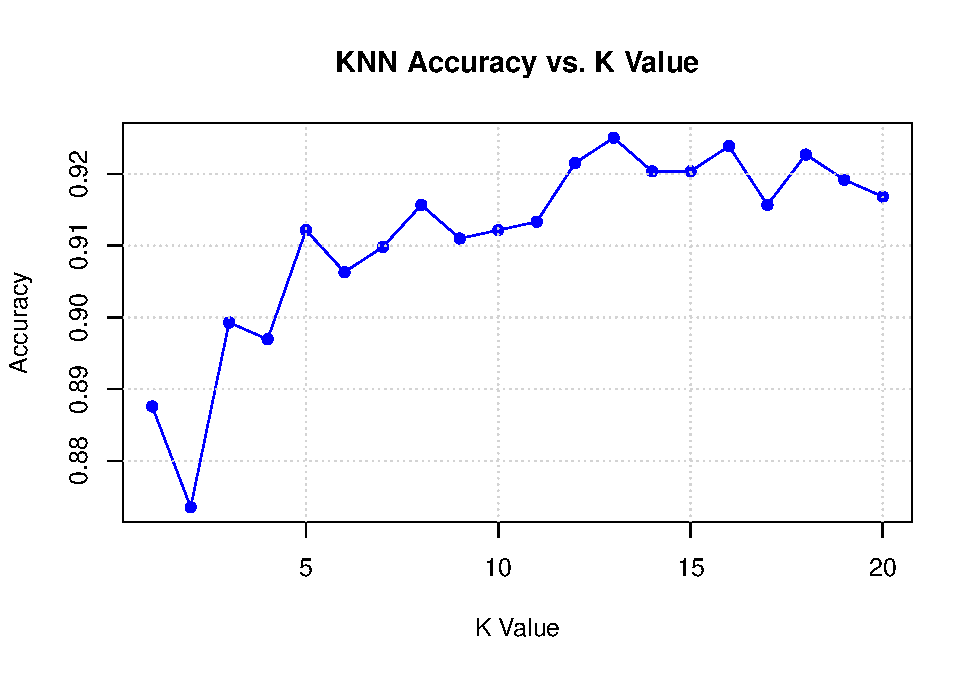
\includegraphics{Loan_approval_files/figure-latex/unnamed-chunk-30-1.pdf}

\#Train KNN Model

\begin{Shaded}
\begin{Highlighting}[]
\CommentTok{\# Load necessary libraries}
\FunctionTok{library}\NormalTok{(class)  }\CommentTok{\# For KNN}
\FunctionTok{library}\NormalTok{(caret)  }\CommentTok{\# For confusionMatrix}
\FunctionTok{library}\NormalTok{(e1071)  }\CommentTok{\# Required for confusionMatrix}

\CommentTok{\# Set seed for reproducibility}
\FunctionTok{set.seed}\NormalTok{(}\DecValTok{65}\NormalTok{)}

\CommentTok{\# Define a function to compute Euclidean distance}
\NormalTok{euclidean\_distance }\OtherTok{\textless{}{-}} \ControlFlowTok{function}\NormalTok{(x1, x2) \{}
  \FunctionTok{sqrt}\NormalTok{(}\FunctionTok{sum}\NormalTok{((x1 }\SpecialCharTok{{-}}\NormalTok{ x2)}\SpecialCharTok{\^{}}\DecValTok{2}\NormalTok{))}
\NormalTok{\}}

\CommentTok{\# Standardize the features to ensure fair distance computation}
\NormalTok{train\_features\_scaled }\OtherTok{\textless{}{-}} \FunctionTok{scale}\NormalTok{(train\_features)}
\NormalTok{test\_features\_scaled }\OtherTok{\textless{}{-}} \FunctionTok{scale}\NormalTok{(test\_features)}

\CommentTok{\# Define K value}
\NormalTok{k\_value }\OtherTok{\textless{}{-}} \DecValTok{13}

\CommentTok{\# Train KNN model with Euclidean distance}
\CommentTok{\#Since knn() in the class package already defaults to Euclidean distance, this ensures that all feature values are standardized before applying KNN, which is important when using distance{-}based algorithms.}

\NormalTok{knn\_pred }\OtherTok{\textless{}{-}} \FunctionTok{knn}\NormalTok{(}\AttributeTok{train =}\NormalTok{ train\_features\_scaled, }
                \AttributeTok{test =}\NormalTok{ test\_features\_scaled, }
                \AttributeTok{cl =}\NormalTok{ train\_labels, }
                \AttributeTok{k =}\NormalTok{ k\_value)}

\CommentTok{\# Convert test labels and predictions to factors with the same levels}
\NormalTok{test\_labels }\OtherTok{\textless{}{-}} \FunctionTok{factor}\NormalTok{(test\_labels, }\AttributeTok{levels =} \FunctionTok{unique}\NormalTok{(train\_labels))}
\NormalTok{knn\_pred }\OtherTok{\textless{}{-}} \FunctionTok{factor}\NormalTok{(knn\_pred, }\AttributeTok{levels =} \FunctionTok{unique}\NormalTok{(train\_labels))}

\CommentTok{\# Create confusion matrix}
\NormalTok{conf\_matrix }\OtherTok{\textless{}{-}} \FunctionTok{confusionMatrix}\NormalTok{(knn\_pred, test\_labels)}

\CommentTok{\# Print full confusion matrix}
\FunctionTok{print}\NormalTok{(conf\_matrix)}
\end{Highlighting}
\end{Shaded}

\begin{verbatim}
## Confusion Matrix and Statistics
## 
##            Reference
## Prediction   Approved  Rejected
##    Approved       490        37
##    Rejected        41       286
##                                           
##                Accuracy : 0.9087          
##                  95% CI : (0.8873, 0.9271)
##     No Information Rate : 0.6218          
##     P-Value [Acc > NIR] : <2e-16          
##                                           
##                   Kappa : 0.8063          
##                                           
##  Mcnemar's Test P-Value : 0.7341          
##                                           
##             Sensitivity : 0.9228          
##             Specificity : 0.8854          
##          Pos Pred Value : 0.9298          
##          Neg Pred Value : 0.8746          
##              Prevalence : 0.6218          
##          Detection Rate : 0.5738          
##    Detection Prevalence : 0.6171          
##       Balanced Accuracy : 0.9041          
##                                           
##        'Positive' Class :  Approved       
## 
\end{verbatim}

\begin{Shaded}
\begin{Highlighting}[]
\CommentTok{\# Extract Accuracy}
\NormalTok{accuracy }\OtherTok{\textless{}{-}}\NormalTok{ conf\_matrix}\SpecialCharTok{$}\NormalTok{overall[}\StringTok{"Accuracy"}\NormalTok{]}
\FunctionTok{print}\NormalTok{(}\FunctionTok{paste}\NormalTok{(}\StringTok{"Accuracy:"}\NormalTok{, }\FunctionTok{round}\NormalTok{(accuracy, }\DecValTok{4}\NormalTok{)))}
\end{Highlighting}
\end{Shaded}

\begin{verbatim}
## [1] "Accuracy: 0.9087"
\end{verbatim}

\begin{Shaded}
\begin{Highlighting}[]
\CommentTok{\# Extract Precision, Recall, and F1{-}score}
\NormalTok{precision }\OtherTok{\textless{}{-}}\NormalTok{ conf\_matrix}\SpecialCharTok{$}\NormalTok{byClass[}\StringTok{"Precision"}\NormalTok{]}
\NormalTok{recall }\OtherTok{\textless{}{-}}\NormalTok{ conf\_matrix}\SpecialCharTok{$}\NormalTok{byClass[}\StringTok{"Recall"}\NormalTok{]}
\NormalTok{f1\_score }\OtherTok{\textless{}{-}}\NormalTok{ conf\_matrix}\SpecialCharTok{$}\NormalTok{byClass[}\StringTok{"F1"}\NormalTok{]}

\FunctionTok{print}\NormalTok{(}\FunctionTok{paste}\NormalTok{(}\StringTok{"Precision:"}\NormalTok{, }\FunctionTok{round}\NormalTok{(precision, }\DecValTok{4}\NormalTok{)))}
\end{Highlighting}
\end{Shaded}

\begin{verbatim}
## [1] "Precision: 0.9298"
\end{verbatim}

\begin{Shaded}
\begin{Highlighting}[]
\FunctionTok{print}\NormalTok{(}\FunctionTok{paste}\NormalTok{(}\StringTok{"Recall:"}\NormalTok{, }\FunctionTok{round}\NormalTok{(recall, }\DecValTok{4}\NormalTok{)))}
\end{Highlighting}
\end{Shaded}

\begin{verbatim}
## [1] "Recall: 0.9228"
\end{verbatim}

\begin{Shaded}
\begin{Highlighting}[]
\FunctionTok{print}\NormalTok{(}\FunctionTok{paste}\NormalTok{(}\StringTok{"F1 Score:"}\NormalTok{, }\FunctionTok{round}\NormalTok{(f1\_score, }\DecValTok{4}\NormalTok{)))}
\end{Highlighting}
\end{Shaded}

\begin{verbatim}
## [1] "F1 Score: 0.9263"
\end{verbatim}

\section{Detailed Model Performance
Insights:}\label{detailed-model-performance-insights}

-Accuracy: 0.9087 - The model correctly predicts loan approval status
for 90.87\% of cases.

-Precision: 0.9298 - When the model predicts loan approval, it's correct
92.98\% of the time.

-Recall: 0.9228 - The model correctly identifies 92.28\% of all actual
approved loans.

-F1-score: 0.9263 - Indicates a good balance between precision and
recall.

-Kappa: 0.8063 - Indicates a very good agreement.

\section{CONCLUSION}\label{conclusion}

The K-Nearest Neighbors (KNN) model developed for loan approval
prediction demonstrates strong performance and reliability:

\begin{enumerate}
\def\labelenumi{\arabic{enumi}.}
\item
  High Accuracy: With an accuracy of 90.87\%, the model shows excellent
  overall predictive capability.
\item
  Balanced Performance: High precision (92.98\%) and recall (92.28\%)
  indicate the model's effectiveness in both approving worthy candidates
  and identifying potential defaults.
\item
  Robust Discrimination: A Balanced Accuracy of 0.9041 suggests the
  model's strong ability to distinguish between approved and rejected
  loan applications.
\item
  Key Factors: The analysis highlighted CIBIL score, income, and loan
  amount as crucial factors in loan approval decisions.
\item
  Practical Applicability: The model's performance suggests it could be
  a valuable tool in assisting loan approval decisions in real-world
  scenarios.
\end{enumerate}

\end{document}
